
\section{Comparison to Observations} 
\label{migration:sec:obs_comp} 

% fig 8
\afterpage{
\clearpage
\begin{landscape}
\begin{figure*} 
\centering 
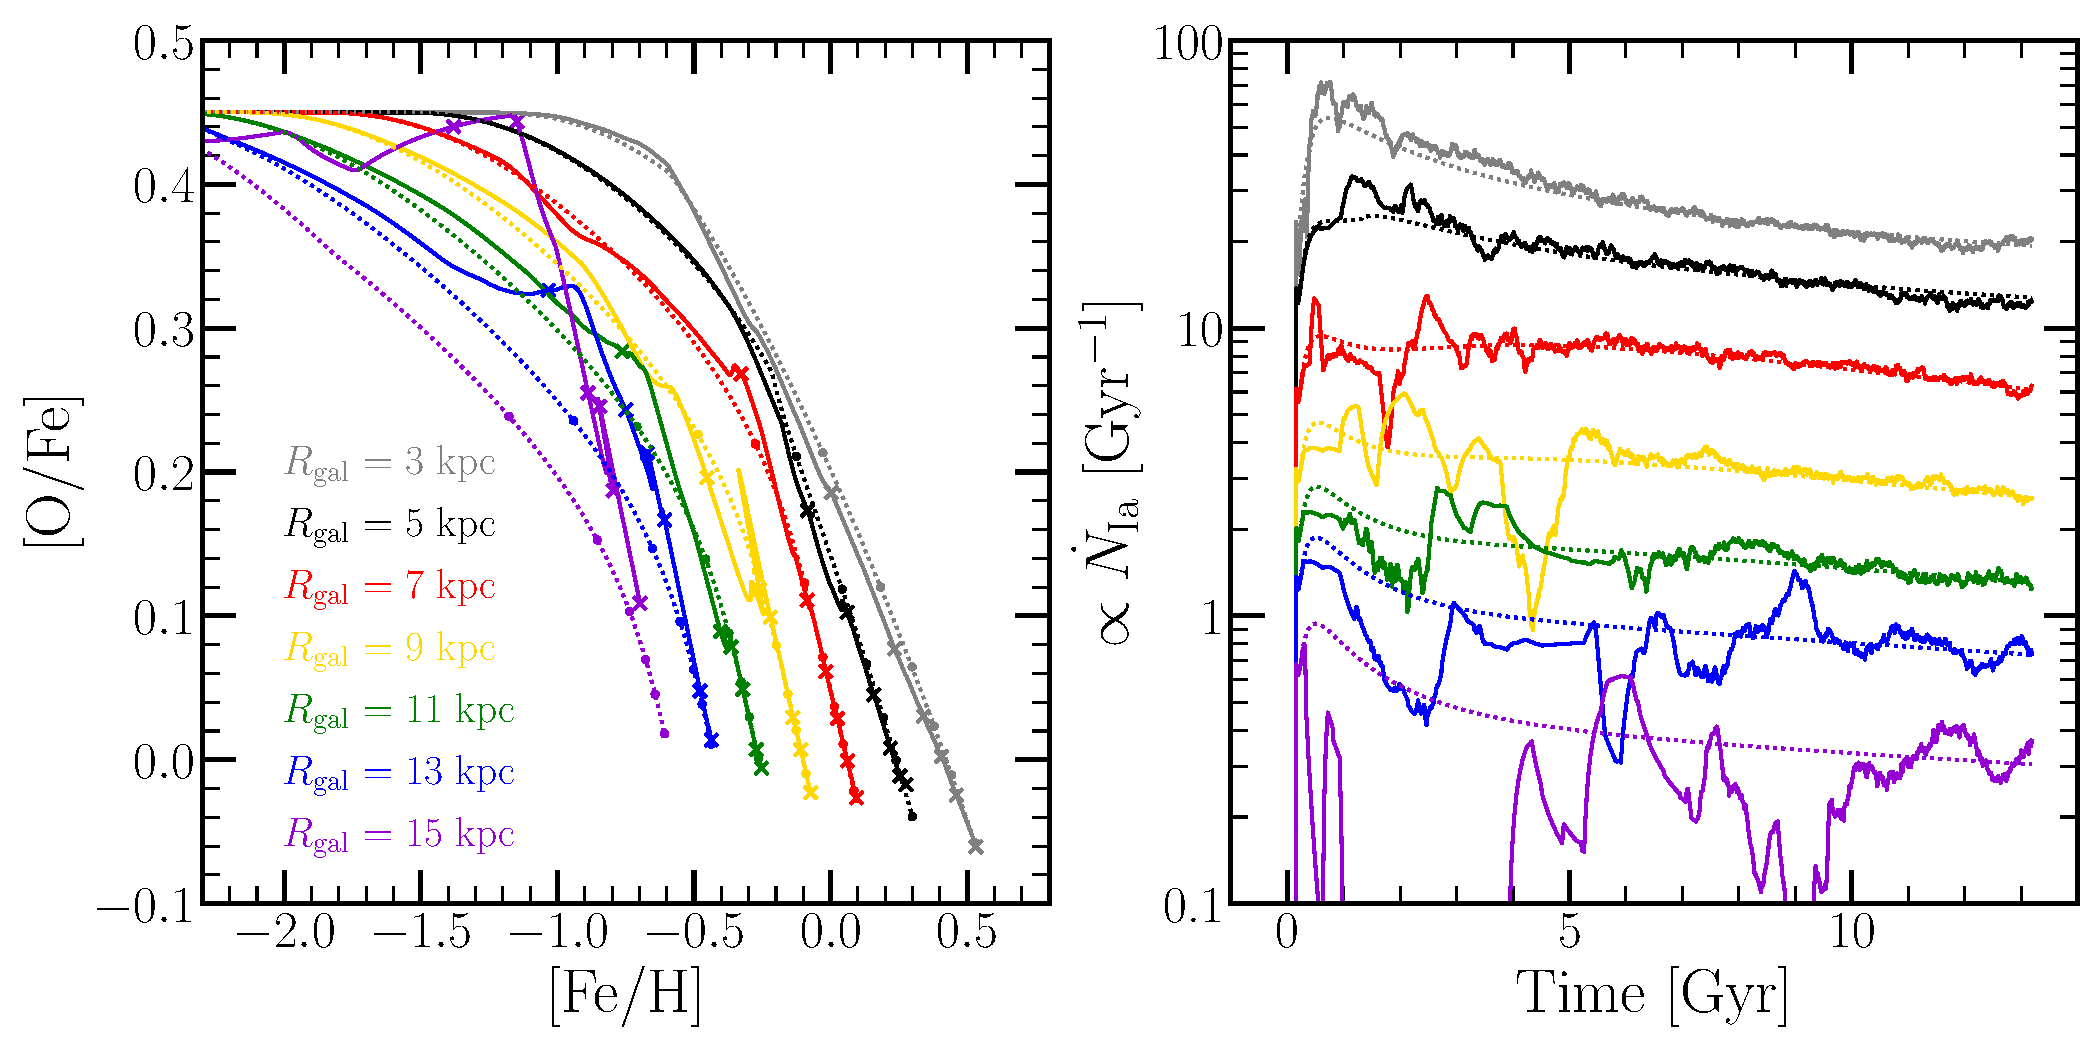
\includegraphics[scale = 0.47]{tracks.pdf} 
\caption{\textbf{Left}: Gas phase evolutionary tracks in the [O/Fe]-[Fe/H] 
plane for our inside-out SFH with either post-processing (dotted lines) or 
diffusion (solid lines) migration models. We plot tracks for seven of our 
$\delta\rgal$ = 100 pc rings, 
colour-coded according to their Galactocentric radius and denoted by the 
legend in the lower-left. We mark simulation times of 2, 4, 6, 8, 10, and 13.2 
Gyr in X's for the diffusion model and points for the post-processing model. 
\textbf{Right}: As a function of simulation time, a proxy for the SN Ia rate 
using the total time-derivative of the Fe mass in a given annulus, calculated 
by subtracting the contribution from recycling and CCSN enrichment and adding 
back that lost to star formation and outflows. We show these rates for the 
same rings as in the left-hand panel, multiplying them by various prefactors 
to improve clarity. } 
\label{migration:fig:tracks} 
\end{figure*} 
\end{landscape}
\clearpage
}

We begin the comparison of our model predictions to observational data with the 
distribution of stellar populations in the [O/Fe]-[Fe/H] plane. We separate 
stars into bins based on their present-day Galactic regions defined by five 
bins in~$R_\text{gal}$ (3 - 5, 5 - 7, 7 - 9, 9 - 11, and 11 - 13 kpc) and three 
bins in~$\left|z\right|$ (0 - 0.5, 0.5 - 1, and 1 - 2 kpc). Within each of the 
resulting 15 regions, we sample 10,000 stars at random from our baseline 
inside-out SFH model. Since stars in~\texttt{VICE} are stand-ins for entire 
stellar populations, we let the probability of sampling one of them be 
proportional to its present day mass. We plot the results of this procedure in 
Fig.~\ref{migration:fig:ofe_feh_diagram}, colour-coding each stellar population by its 
birth radius; for visual reference, we also plot the gas-phase track which 
resulted from the~$R_\text{gal}$ = 8 kpc annulus with the post-processing 
migration model in a black solid line in all panels. 
\par 
In Fig.~\ref{migration:fig:ofe_feh_diagram}, we note that high-$\alpha$~sequence stars 
are predicted to be the dominant population at small~$R_\text{gal}$ and high 
$\left|z\right|$; conversely, the low-$\alpha$~population dominates the 
statistics at large~$R_\text{gal}$~and low~$\left|z\right|$. This is consistent 
with the observational results of~\citet{Hayden2015}, who present a density map 
in the [$\alpha$/M]-[M/H] plane for the same Galactic regions (see their Fig. 
4).\footnote{
	In~\citet{Hayden2015}, [M/H] represents an overall scaling of elements with 
	solar mixture, and [$\alpha$/M] represents a scaling of~$\alpha$-elements 
	with respect to others. To a good approximation they are proxies for 
	[Fe/H] and [O/Fe], respectively, and we will treat them as such in this 
	paper. 
} 
Furthermore, the locus of the low-$\alpha$ sequence shifts from super-solar 
[Fe/H] to sub-solar [Fe/H] with increasing~$R_\text{gal}$, a shift which is 
expected given the abundance gradient that we have built into our models (see 
discussion in~\S~\ref{migration:sec:methods:outflows}). 
The colour-coding of the points 
shows that the width of the low-$\alpha$~sequence arises out of 
stellar migration: low-$\alpha$ stars with high [Fe/H] formed in the inner 
Galaxy, and those with low [Fe/H] formed in the outer Galaxy. 
The low-$\alpha$ locus thus represents a superposition of populations achieved 
by radial migration rather than an evolutionary sequence, the interpretation 
proposed by, e.g.,~\citet{Schoenrich2009a} and~\citet{Nidever2014}. 
\par 
In Fig.~\ref{migration:fig:ofe_feh_diagram} one can clearly see the imprint of 
evolutionary tracks from different radii, appearing in the same present-day 
$R_\text{gal}$ bin because of radial mixing. 
Though this is to some extent a consequence of the discretization of the 
Galaxy disc in our model, it also arises out of correlated fluctuations in the 
SN Ia rate (see discussion in~\S~\ref{migration:sec:obs_comp:gradient}). 
Observational scatter would wash out the appearance of distinct tracks, and 
intrinsic scatter might blur them if our chemical evolution model was less 
idealized. 
Our model reproduces several of the qualitative trends found by 
\citet{Hayden2015}, but the distribution is less obviously bimodal. 
We quantify this point in~\S~\ref{migration:sec:obs_comp:ofe_dists} below. 
If we remake Fig.~\ref{migration:fig:ofe_feh_diagram} for any of our other SFHs, or for 
our alternative migration or star formation efficiency prescriptions, the 
appearance is qualitatively similar. There are significant quantitative 
differences in some cases, which we discuss in subsequent subsections. 

\subsection{Abundance Gradients} 
\label{migration:sec:obs_comp:gradient} 

% fig 9 
\afterpage{
\clearpage
\begin{landscape}
\begin{figure*} 
\centering 
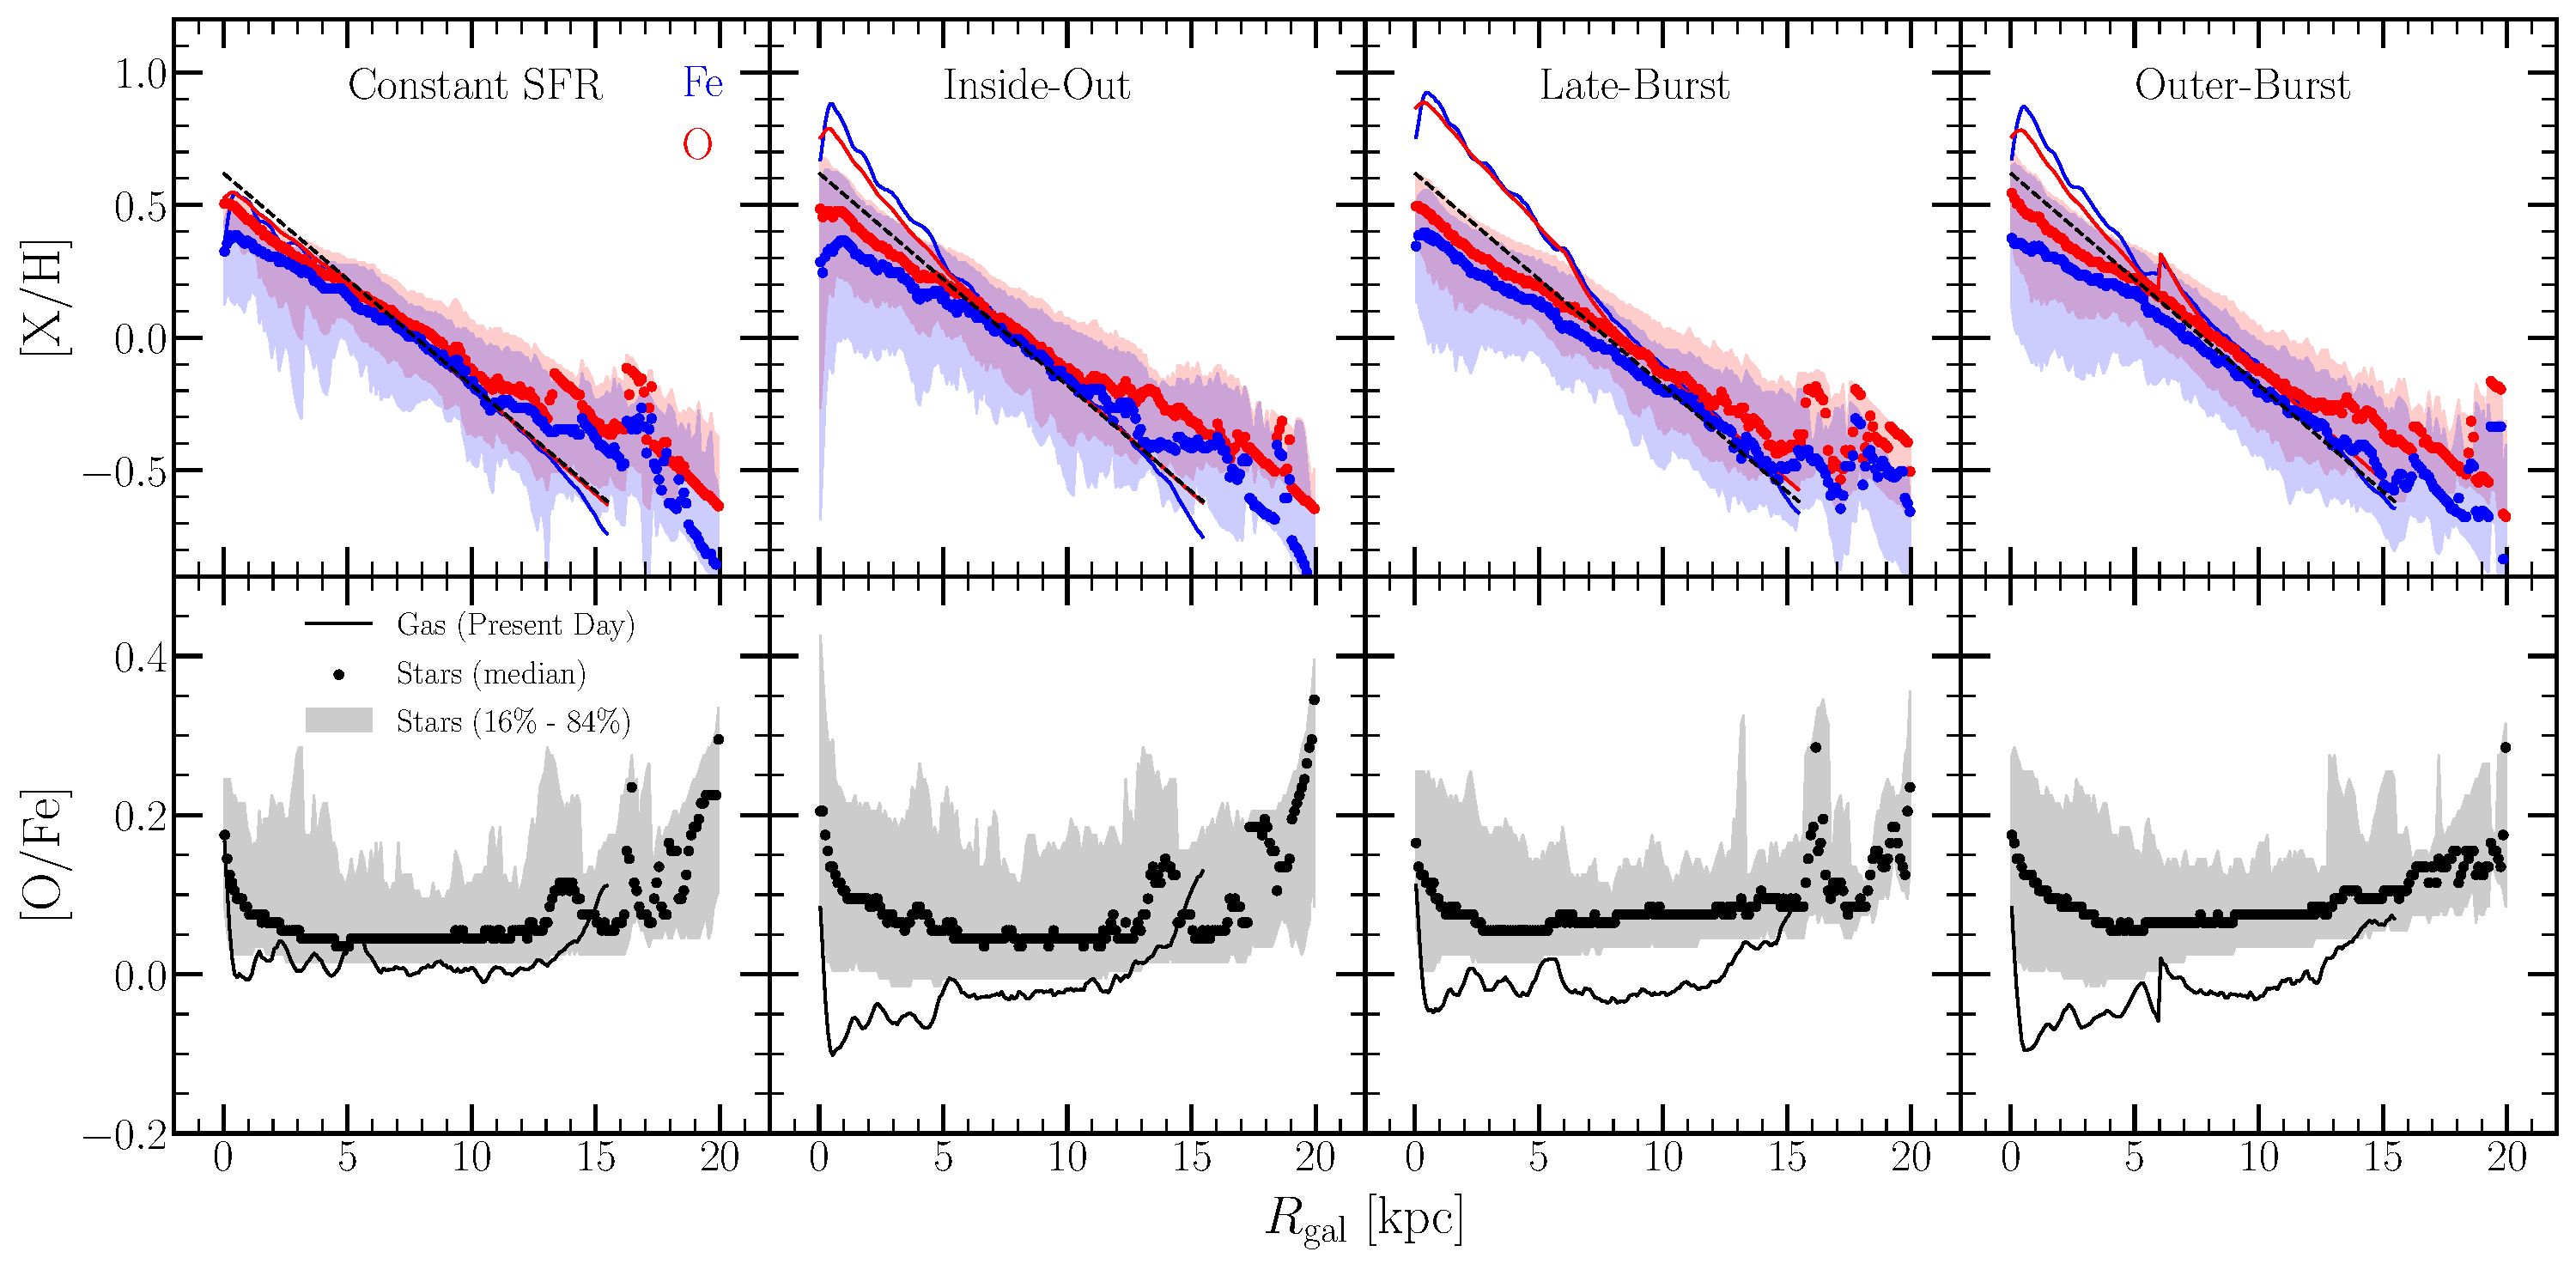
\includegraphics[scale = 0.38]{metallicity_gradient.pdf} 
\caption{Radial abundance gradients in [O/H] (top, red), [Fe/H] (top, blue), 
and [O/Fe] (bottom) for our four SFHs with diffusion migration - constant (far 
left), inside-out (left-middle), late-burst (right-middle), and outer-burst 
(far right). We plot the gas-phase abundance at the present day as a function 
of Galactocentric radius in solid lines. Points denote the median of the stellar 
MDF of the 100-pc width ring at a given radius, with shaded regions marking 
the 16th and 84th percentiles thereof. Black lines in the top panels denote our 
target [$\alpha$/H] gradient of mode([$\alpha$/H]) = +0.3 at~$R_\text{gal}$~= 
4 kpc with a slope of -0.08 kpc$^{-1}$. } 
\label{migration:fig:metallicity_gradient} 
\end{figure*} 
\end{landscape}
\clearpage
}

The left panel of Fig.~\ref{migration:fig:tracks} shows gas phase [O/Fe]-[Fe/H] 
evolutionary tracks at several radii assuming the inside-out SFH, using either 
our post-processing (dotted) or diffusion (solid) migration prescriptions 
(see~\S~\ref{migration:sec:methods:migration} and Fig.~\ref{migration:fig:migration_schema}). 
For the post-processing model the tracks are smooth and simply follow the 
predictions of one-zone GCE models with the parameters appropriate to each 
radius --- with post-processing, radial migration has no impact on the gas-phase 
evolution. 
However, some of the tracks in the diffusion model are notably 
different, especially at early times and large radii. 
These differences arise because radial migration can transport stars 
significantly over the timescale of SN Ia enrichment, as discussed in~\S 
\ref{migration:sec:methods:h277}.
\par 
To demonstrate this point, the right panel of Fig.~\ref{migration:fig:tracks} plots a 
proxy of the SN Ia rate\footnote{
	From our~\vice~outputs, the total time derivative of the Fe mass in a given 
	annulus can be obtained by its change across a single timestep. By then 
	subtracting the CCSN contribution (known exactly given our adopted yield 
	and the SFR), approximately correcting for recycling, and adding back that 
	which was lost to star formation and outflows, we obtain a simple estimate 
	of Fe production by SNe Ia. 
} as a function of time for the same 0.1 kpc rings plotted in the left panel. 
At large radii the sources for the diffusion model exhibit large fluctuations 
relative to the smooth predictions of the underlying one-zone models, as 
migration boosts or depletes the predicted number of SN Ia progenitors. 
The deficits or excesses in SN Ia rate in turn drive upward or downward 
deviations in [O/Fe] relative to the smooth model tracks in the left panel. 
As an extreme example, in the 15 kpc annulus the SN Ia rate is nearly zero for 
the first~$\sim$3 Gyr, and its resulting [O/Fe] track is nearly flat over this 
interval, even though the smooth model track has dropped from [O/Fe] = 0.45 to 
[O/Fe]~$\approx$ 0.2. 
Although we illustrate the SN Ia rates for only a handful of rings, we have 
found that the variations between nearby rings are highly correlated in our 
models, suggesting that regions of the Galaxy move coherently in 
[O/Fe]-[Fe/H] space; this lends further insight into the streak-like appearance 
of some sub-populations in Fig.~\ref{migration:fig:ofe_feh_diagram}. 
\par 
Because we are analyzing a single hydrodynamic simulation, we cannot say 
whether the systematic depression of the SN Ia rate at large radii and early 
times is a general expectation or a consequence of the specific dynamical 
history of this galaxy. 
However, greater fluctuations at large~\rgal~and small~$t$ are a natural 
consequence of the low SFR. These fluctuations can have a significant impact 
on [O/Fe]-[Fe/H] evolution even if their sign varies from galaxy to galaxy. 
The fact that >10\% of events are seen at >10 kpc from their host galaxies in 
the ASAS-SN bright SN catalog~\citep{Holoien2019} adds qualitative 
observational support to the argument that SN Ia progenitors may often form at 
significantly different radii than where their explosions are observed. 
We will show below that these SN Ia rate fluctuations lead to the formation of 
$\alpha$-enhanced intermediate age populations that do not arise in our 
post-processing radial migration model (see Fig.~\ref{migration:fig:age_alpha}). 
\par 
Fig.~\ref{migration:fig:metallicity_gradient} plots the radial gradients of gas phase 
and stellar abundances, [O/H], [Fe/H], and [O/Fe], for our four SFH models. 
For constant SFR, the gas phase abundances closely track the target gradient 
that we used to set our~$\eta(\rgal)$ profile (see equation~\ref{migration:eq:eta_rgal}). 
For a declining SFR the equilibrium abundance is higher than that assumed for 
equation~\refp{migration:eq:eta_rgal}~\citep[see][]{Weinberg2017b}, and in the inside-out 
and outer-burst models the gas phase abundances rise above the target gradient 
at small~\rgal~where the decline is fastest. 
In the late-burst model the inner Galaxy abundances are further boosted by 
enhanced late-time star formation, and a similar effect is seen at~\rgal~= 6 
kpc in the outer-burst model. 
In accretion-induced starbursts, re-enrichment can briefly produce 
super-equilibrium abundances in the gas-phase, which then decay back to the 
equilibrium abundance as the SFR declines~\citep{Johnson2020}. 
\par 
The stellar metallicity gradients are shallower than in the gas phase, and 
they are similar in the four models. 
The 16th-84th percentile range at each radius is large, typically 0.3-0.5 
dex, and typically larger in [Fe/H] than [O/H]. 
The mode of the stellar metallicity distribution is a noisy quantity in our 
0.1-kpc rings, so points in Fig.~\ref{migration:fig:metallicity_gradient} show the 
median of the distributions. 
The trends for the mode are slightly steeper, as expected given the change in 
shape of the metallicity distribution functions (see~\S 
\ref{migration:sec:obs_comp:mdfs}), and closer to the target gradient shown by the black 
solid line. We do not include observational data in this figure, but the target 
gradient itself is observationally motivated, so Fig. 
\ref{migration:fig:metallicity_gradient} implies that our models, by design, give a 
reasonable match to Milky Way abundance gradients. 
\par 
Median [O/Fe] values are close to solar at nearly all radii, rising at the 
smallest~\rgal~and in some models at the largest~\rgal. However, the spread in 
[O/Fe] is large at all radii, and typical values depend on~\absz~and [Fe/H] as 
shown in Fig.~\ref{migration:fig:ofe_feh_diagram}. 
We present a comparison to observations in~\S~\ref{migration:sec:obs_comp:ofe_dists} 
below. 
The larger values of [O/Fe] beyond~\rgal~= 15.5 kpc are expected, since this is 
the radius at which we shut off star formation. In our models, all stellar 
populations at these radii migrated there, so they tend to be old and therefore 
$\alpha$-enhanced. 
The idea that outer disc populations are dominated by migration was proposed 
by~\citet{Roskar2008b} based on simulation predictions. 
\citet{RadburnSmith2012} present observational evidence for this prediction in 
the observations of the NGC 7793 disc. 
Although we are not modeling the bulge in this paper, our model predicts the 
disc stars in these regions to have higher [O/Fe] than at larger~\rgal, in 
qualitative agreement with observations (see discussion in, e.g., 
\citealp{Duong2019, Griffith2021a}). 

\subsection{Metallicity Distribution Functions} 
\label{migration:sec:obs_comp:mdfs} 

% fig 10 
\begin{figure} 
\centering 
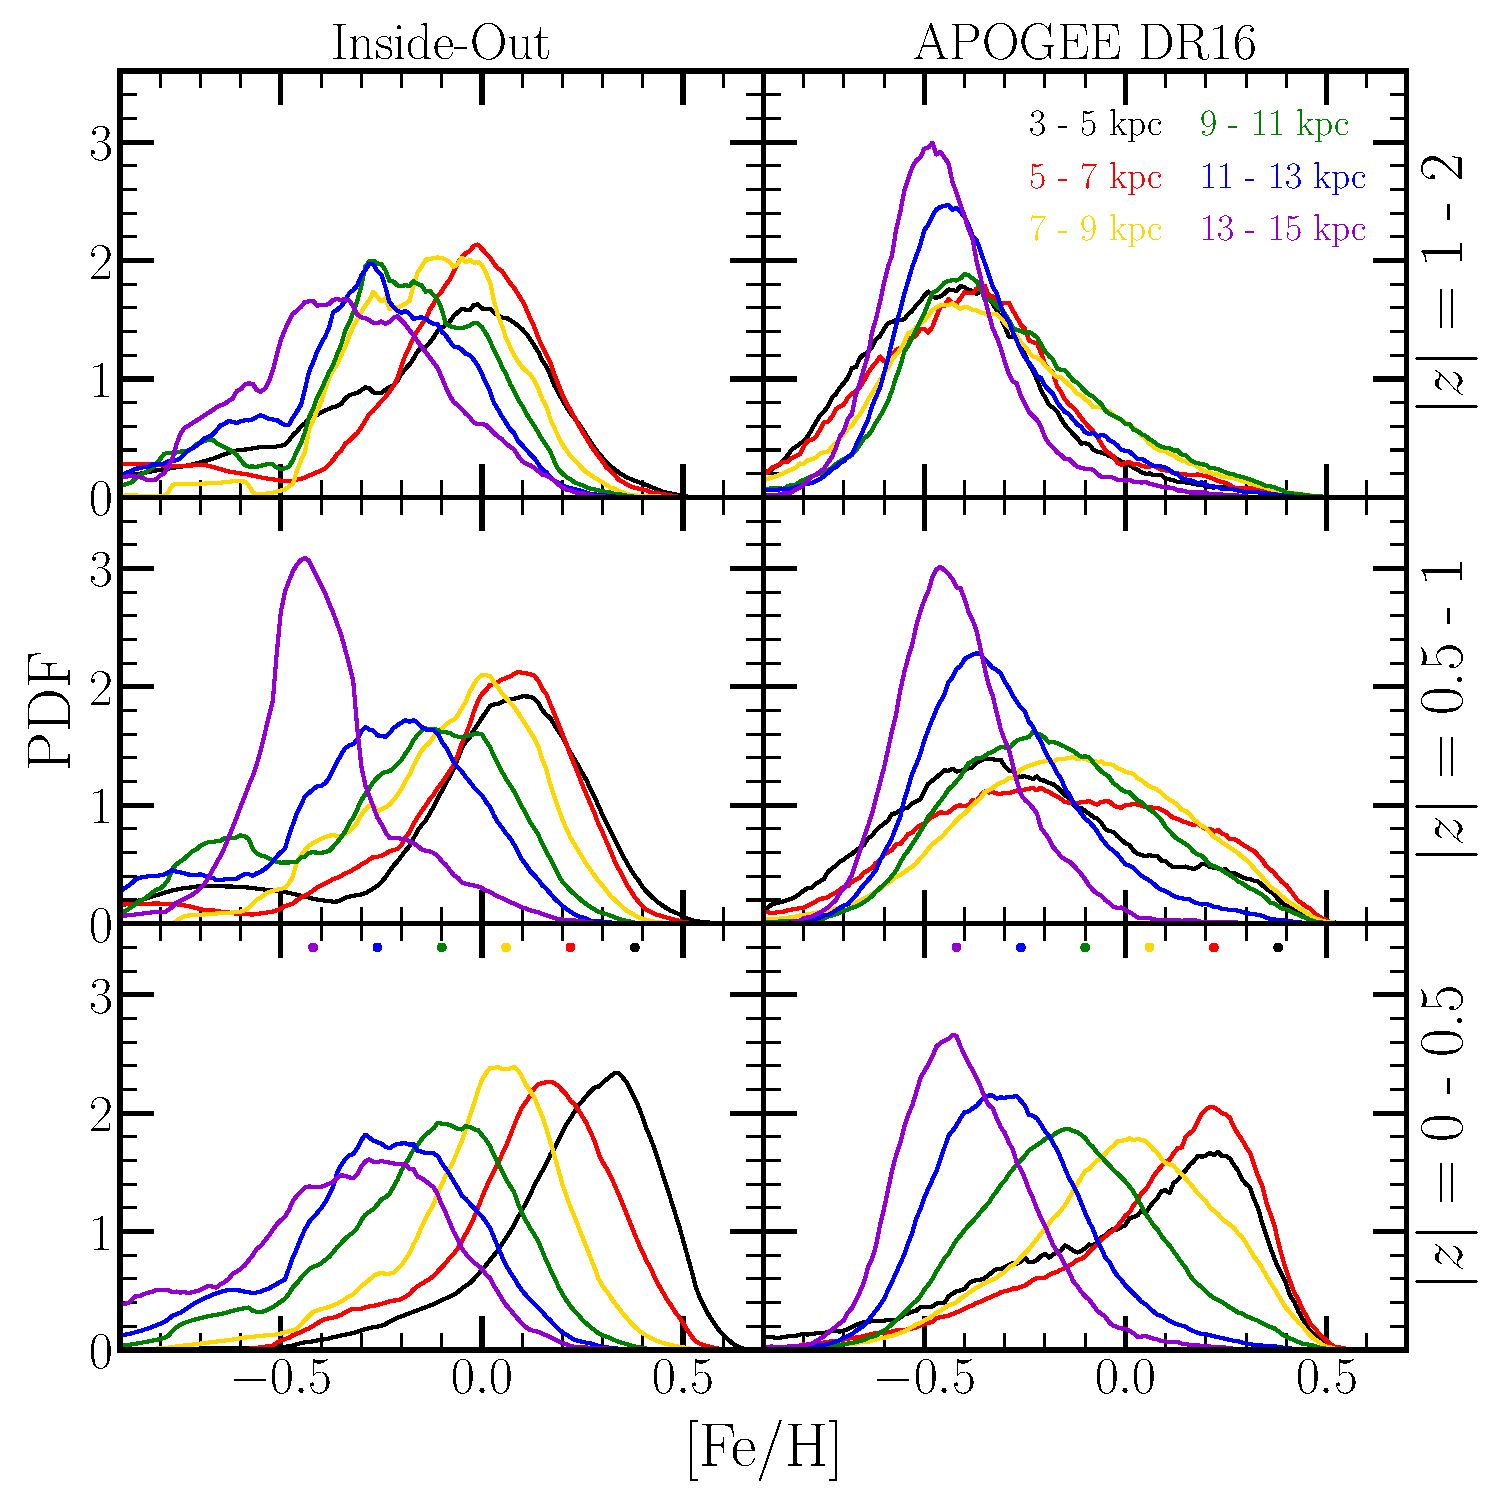
\includegraphics[scale = 0.45]{mdf_3panel_fe.pdf} 
\caption{Metallicity distribution functions (MDFs) in [Fe/H] predicted by our 
fiducial, inside-out model (left) and as observed in APOGEE DR16 (right), for 
stars and simulated stellar populations with present-day~$\left|z\right|$~= 0 - 
0.5 kpc (bottom), 0.5 - 1 kpc (middle), and 1 - 2 kpc (top). MDFs are shown in 
bins of Galactocentric radius: 3 - 5 kpc (black), 5 - 7 kpc (red), 7 - 9 kpc 
(yellow), 9 - 11 kpc (green), 11 - 13 kpc (blue), and 13 - 15 kpc (purple). 
The points near the top of the bottom panels denote what the mode abundance 
would be if it followed out target gradient of [Fe/H] = +0.3 at~$R_\text{gal}$ 
= 4 kpc with a slope of -0.08 kpc$^{-1}$ exactly, assuming the inner radius of 
each bin (i.e. there is no point plotted for 15 kpc). All distributions are 
smoothed with a box-car width of [Fe/H]~$\pm$~0.1 for clarity. } 
\label{migration:fig:mdf_3panel_fe} 
\end{figure} 

% fig 11 
\begin{figure} 
\centering 
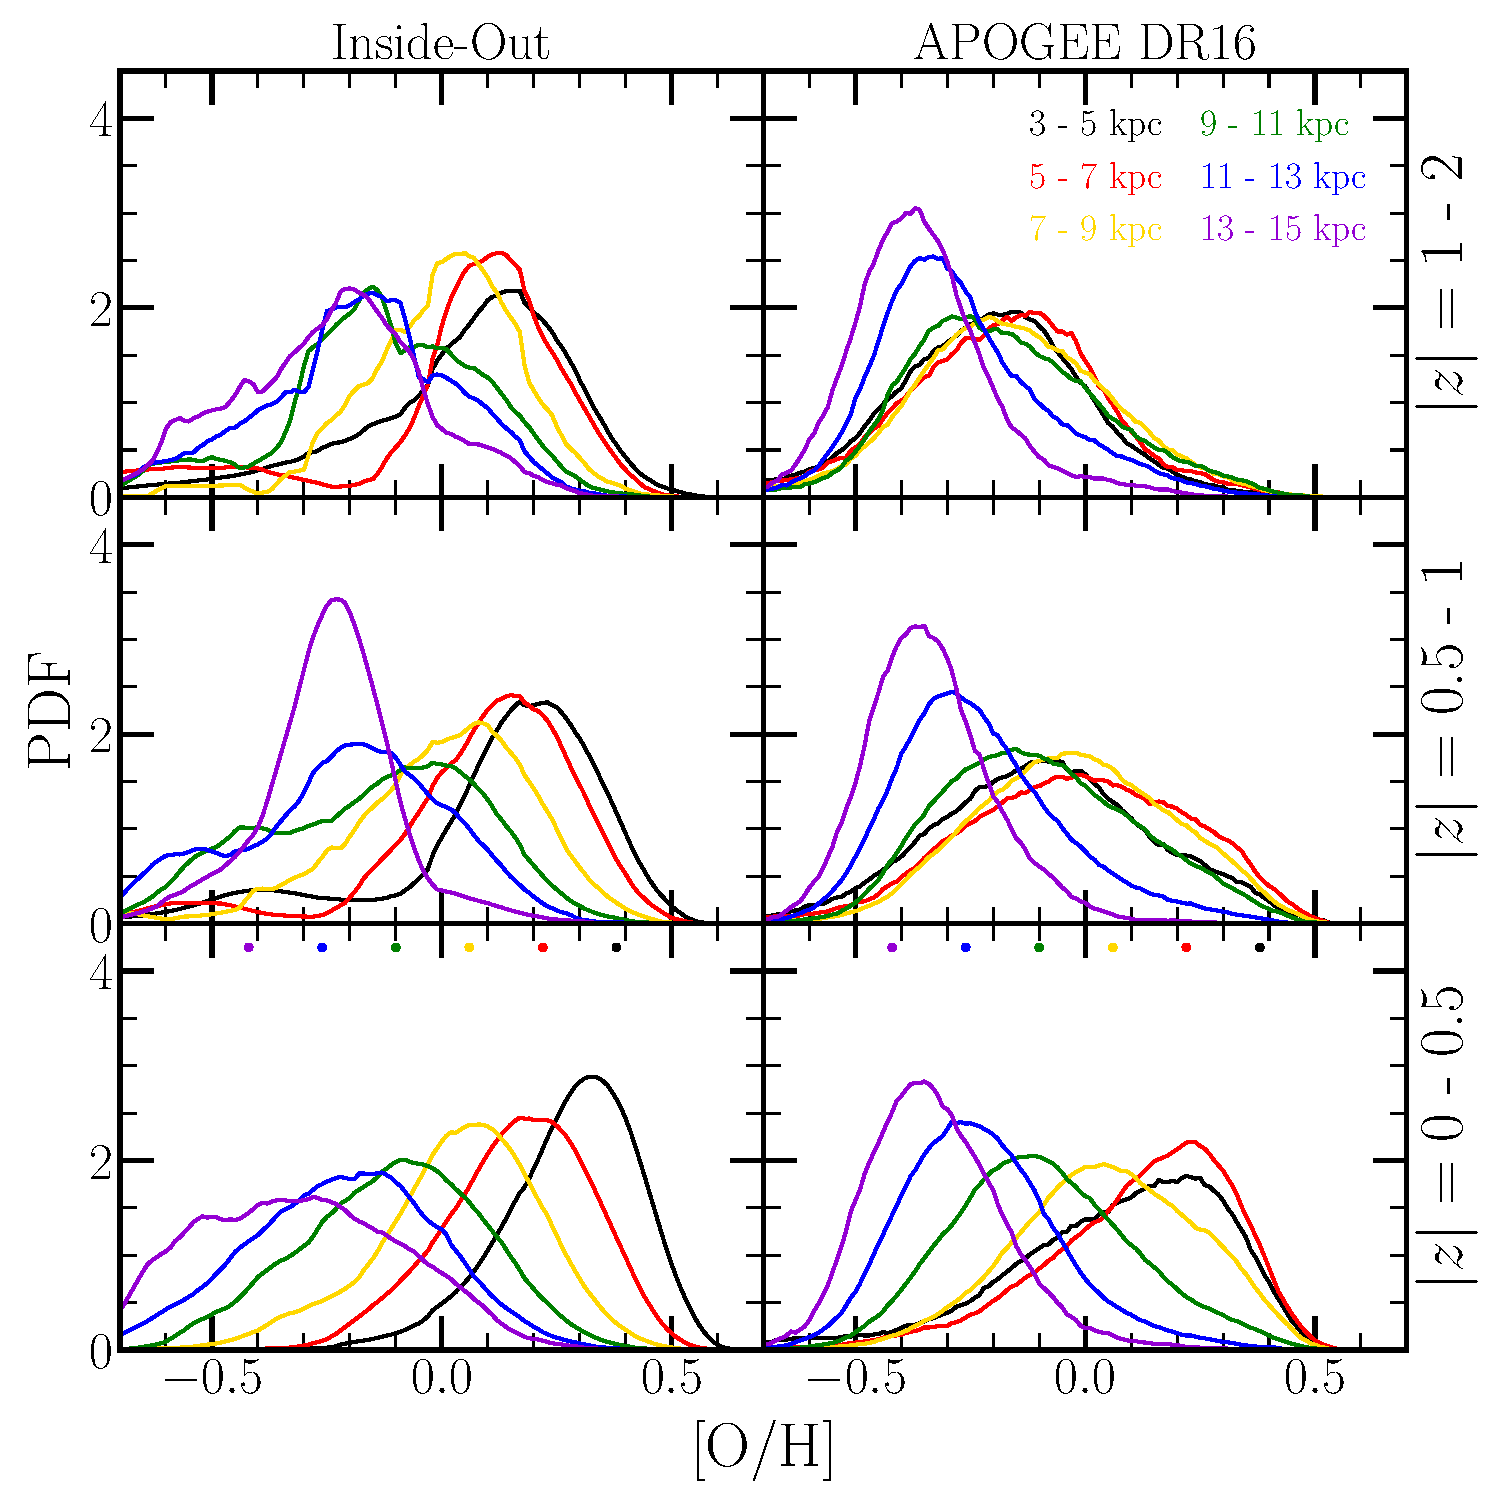
\includegraphics[scale = 0.45]{mdf_3panel_o.pdf} 
\caption{The same as Fig.~\ref{migration:fig:mdf_3panel_fe}, but for [O/H]. } 
\label{migration:fig:mdf_3panel_o} 
\end{figure} 

Metallicity distribution functions (MDFs) and their variations with Galactic 
region are a core prediction of GCE models. 
We have computed distributions of [Fe/H] and [O/H] using abundances from the 
16th data release~\citep[DR16;][]{Ahumada2020, Joensson2020} of APOGEE 
\citep{Majewski2017}. 
Abundances are determined by the APOGEE Stellar Parameters and Chemical 
Abundances Pipeline (ASPCAP;~\citealp{Holtzman2015, GarciaPerez2016}). 
We restrict our sample to stars with effective temperatures of 4000 K 
$\leq T_\text{eff} \leq$~4600 K, surface gravities of 1.0~$\leq \log g \leq$ 
2.5, and signal-to-noise ratios of at least 100. 
These cuts ensure that our sample consists of stars on the upper red giant 
branch, luminous enough to cover all regions of the disc, while excluding red 
clump stars to avoid possible abundance offsets between these stars and stars 
on the giant branch. 
Our observational results are similar to those shown by~\citet{Hayden2015}, 
but we use a larger data set, more recent APOGEE observations, and [O/H] and 
[Fe/H] rather than [$\alpha$/H] and [M/H]. 
\par 
The left and right panels of Fig.~\ref{migration:fig:mdf_3panel_fe} show [Fe/H] 
distributions from our fiducial inside-out model and the APOGEE data, 
respectively, in bins of~\rgal~and~\absz. 
The observed midplane distributions (\absz~$\leq$~0.5 kpc) show the striking 
phenomenon first noted by~\citet{Hayden2015}: a shift from a skew-negative form 
in the inner Galaxy to a skew-positive form in the outer Galaxy, with a roughly 
symmetric [Fe/H] distribution at the solar circle. 
The simulation reproduces this behaviour, confirming that realistic radial 
migration can explain the radial dependence of the MDF shape as conjectured by 
\citet{Hayden2015} and illustrated in a more idealized simulation by 
\citet{Loebman2016}. 
\par 
In detail, the MDFs are not as smooth at large~\rgal~as in the observations; 
they are not as skewed in the inner and outer disc either. 
Dots in the lower left panel mark the target metallicities implied by our 
$\eta(\rgal)$ prescription in equation~\refp{migration:eq:eta_rgal}. 
The modes of the stellar MDFs track these targets quite closely, except at 
\rgal~= 13 - 15 kpc, where the migrated population is so large compared to the 
in-situ population that it reshapes the peak of the MDF as well as the tails. 
The model also predicts a continuing increase of the mode metallicity down to 
\rgal~= 3 - 5 kpc, while the observed mode is the same at 3 - 5 kpc and 5 - 7 
kpc. 
We do not view this as a serious discrepancy, as it could be reduced by a
moderate adjustment of the~$\eta(\rgal)$ recipe so that the metallicity 
gradient in these regions is flat. 
We have computed such a comparison case and find that it does indeed reproduce 
this observational result, though it still underpredicts the skewness at 
small~\rgal. 
% {\color{red} 
It is also possible that the differences at 3 - 5 kpc are due to stars 
associated with the Milky Way's strong bar, which~\citet{Bovy2019} demonstrate 
to be low metallicity (see their Fig. 5). 
With only a weak and transient bar in~\hsim, this is a dynamical effect not 
included in our models (see discussion in~\S~\ref{migration:sec:methods:h277}). 
% It's also possible that the differences at 3 - 5 kpc are due to low metallicity 
% bar stars in the data~\citep[e.g. those observed by][]{Bovy2019}, a dynamical 
% effect not present in~\hsim~(see discussion in~\S~\ref{migration:sec:methods:h277}). 
% }
Alternatively, the flattening of the observed gradient could be a consequence 
of more aggressive quenching of star formation than assumed in our models. 
The surface density of star formation~$\dot{\Sigma}_\star$ in the Milky Way 
is known to reach a maximum at~\rgal~$\approx$ 4 kpc and decline by a factor 
of a few at smaller radii (see Fig. 1 of~\citealp{Peek2009} and Fig. 2 
of~\citealp{Fraternali2012} and data therein). 
Early quenching could cutoff the MDF at high [O/H] and [Fe/H] if it happens 
before the ISM reaches equilibrium abundance. 
Visual inspection of Fig.~\ref{migration:fig:tracks} suggests that this process should 
occur around~$T \approx$ 6 - 8 Gyr if the MDF is to peak at 
[Fe/H]~$\approx$~+0.2 - 0.3. 
\par 
Going up from the midplane, the observed MDFs for the four inner annuli 
(\rgal~< 11 kpc) shift to lower average metallicity, and they converge in 
location and in shape, being roughly symmetric at~\absz~= 0.5 - 1 kpc and 
mildly skew-positive at~\absz~= 1 - 2 kpc. 
Qualitatively, the simulation reproduces this shift of mean metallicity, change 
of shape, and convergence of distributions at different~\rgal, although the 
model does not account for the entirety of the effect. 
We consider this a significant success of this simulation-based approach 
because our GCE model is constructed and tuned in~\rgal~alone, so trends with 
\absz~follow from the combinations of age-metallicity trends, age-velocity 
trends arising from ``upside-down'' disc formation and dynamical heating, and 
correlations between radial migration and vertical energy. 
\citet{Freudenburg2017} showed that chemical evolution in a vertically settling 
gas disc could explain the MDF trend with~\absz~seen by APOGEE in the inner 
disc, and here we see similar behaviour in a more fully ab initio model. 
\citet{Bird2021} showed that the dynamics of the~\hsim~simulation leads to good 
agreement with the observed age-velocity relation, and here we show that 
this success extends qualitatively to the vertical trends of chemical 
abundances. 
\par 
Quantitatively, there are significant differences between the predicted and 
observed distributions above the midplane. 
The model MDFs from~\absz~= 0.5 - 1 kpc are narrower and more skewed than the 
observed MDFs, with higher median [Fe/H]. 
At~\absz~= 1 - 2 kpc, the predicted MDFs are not as strikingly converged as the 
observed MDFs. 
In both the data and the model, the high-\absz~MDFs for the 11 - 13 and 13 - 15 
kpc annuli remain closer to their midplane counterparts. 
The model [O/Fe]-[Fe/H] distributions in the outer Galaxy appear to show the 
imprint of a few large migration episodes (see Fig.~\ref{migration:fig:ofe_feh_diagram}). 
The smoothness of the observed MDFs at these radii and their similarity across 
\absz~suggests a more vigorous stirring. 
\par 
Fig.~\ref{migration:fig:mdf_3panel_o} plots distributions of [O/H] instead of [Fe/H]. 
The appearance is quite similar to Fig.~\ref{migration:fig:mdf_3panel_fe}, which is 
unsurprising but non-trivial given the different timescales of CCSN and SN Ia 
enrichment. 
The agreement and disagreement between the model and data are similar, though 
the discrepancy for~\absz~= 0.5 - 1 kpc is somewhat clearer in [O/H]. 
The model's outer Galaxy MDFs are less irregular in [O/H] than in [Fe/H], an 
indication that some of the structure in the [Fe/H] distributions is caused by 
the large fluctuations in the SN Ia rate as seen in Fig.~\ref{migration:fig:tracks}. 
We have confirmed this conjecture by computing [Fe/H] MDFs for the 
post-processing radial migration prescription, finding that they are indeed 
more smooth at~\rgal~= 11 kpc. 
\par 
The MDF predictions for our other SFH scenarios - constant SFR, late-burst, and 
outer-burst - are different in detail, but they show the same qualitative 
trends as those in Figs.~\ref{migration:fig:mdf_3panel_fe} and~\ref{migration:fig:mdf_3panel_o}. 
Our findings on the radial and vertical trends of the MDF are also similar 
to those of~\citet{Loebman2016}, who use a galaxy simulation evolved from 
rotating gas in a dark matter halo rather than cosmological initial conditions. 
The qualitative similarity of our results across different models implies that 
the radial and vertical trends are a generic effect of radial migration, 
upside-down disc formation, and dynamical heating in a galaxy with realistic 
abundance gradients and time evolution. 


\subsection{[O/Fe] distributions in Bins of [Fe/H]} 
\label{migration:sec:obs_comp:ofe_dists} 

% fig 12 
\afterpage{
\clearpage
\begin{landscape}
\begin{figure*} 
\centering 
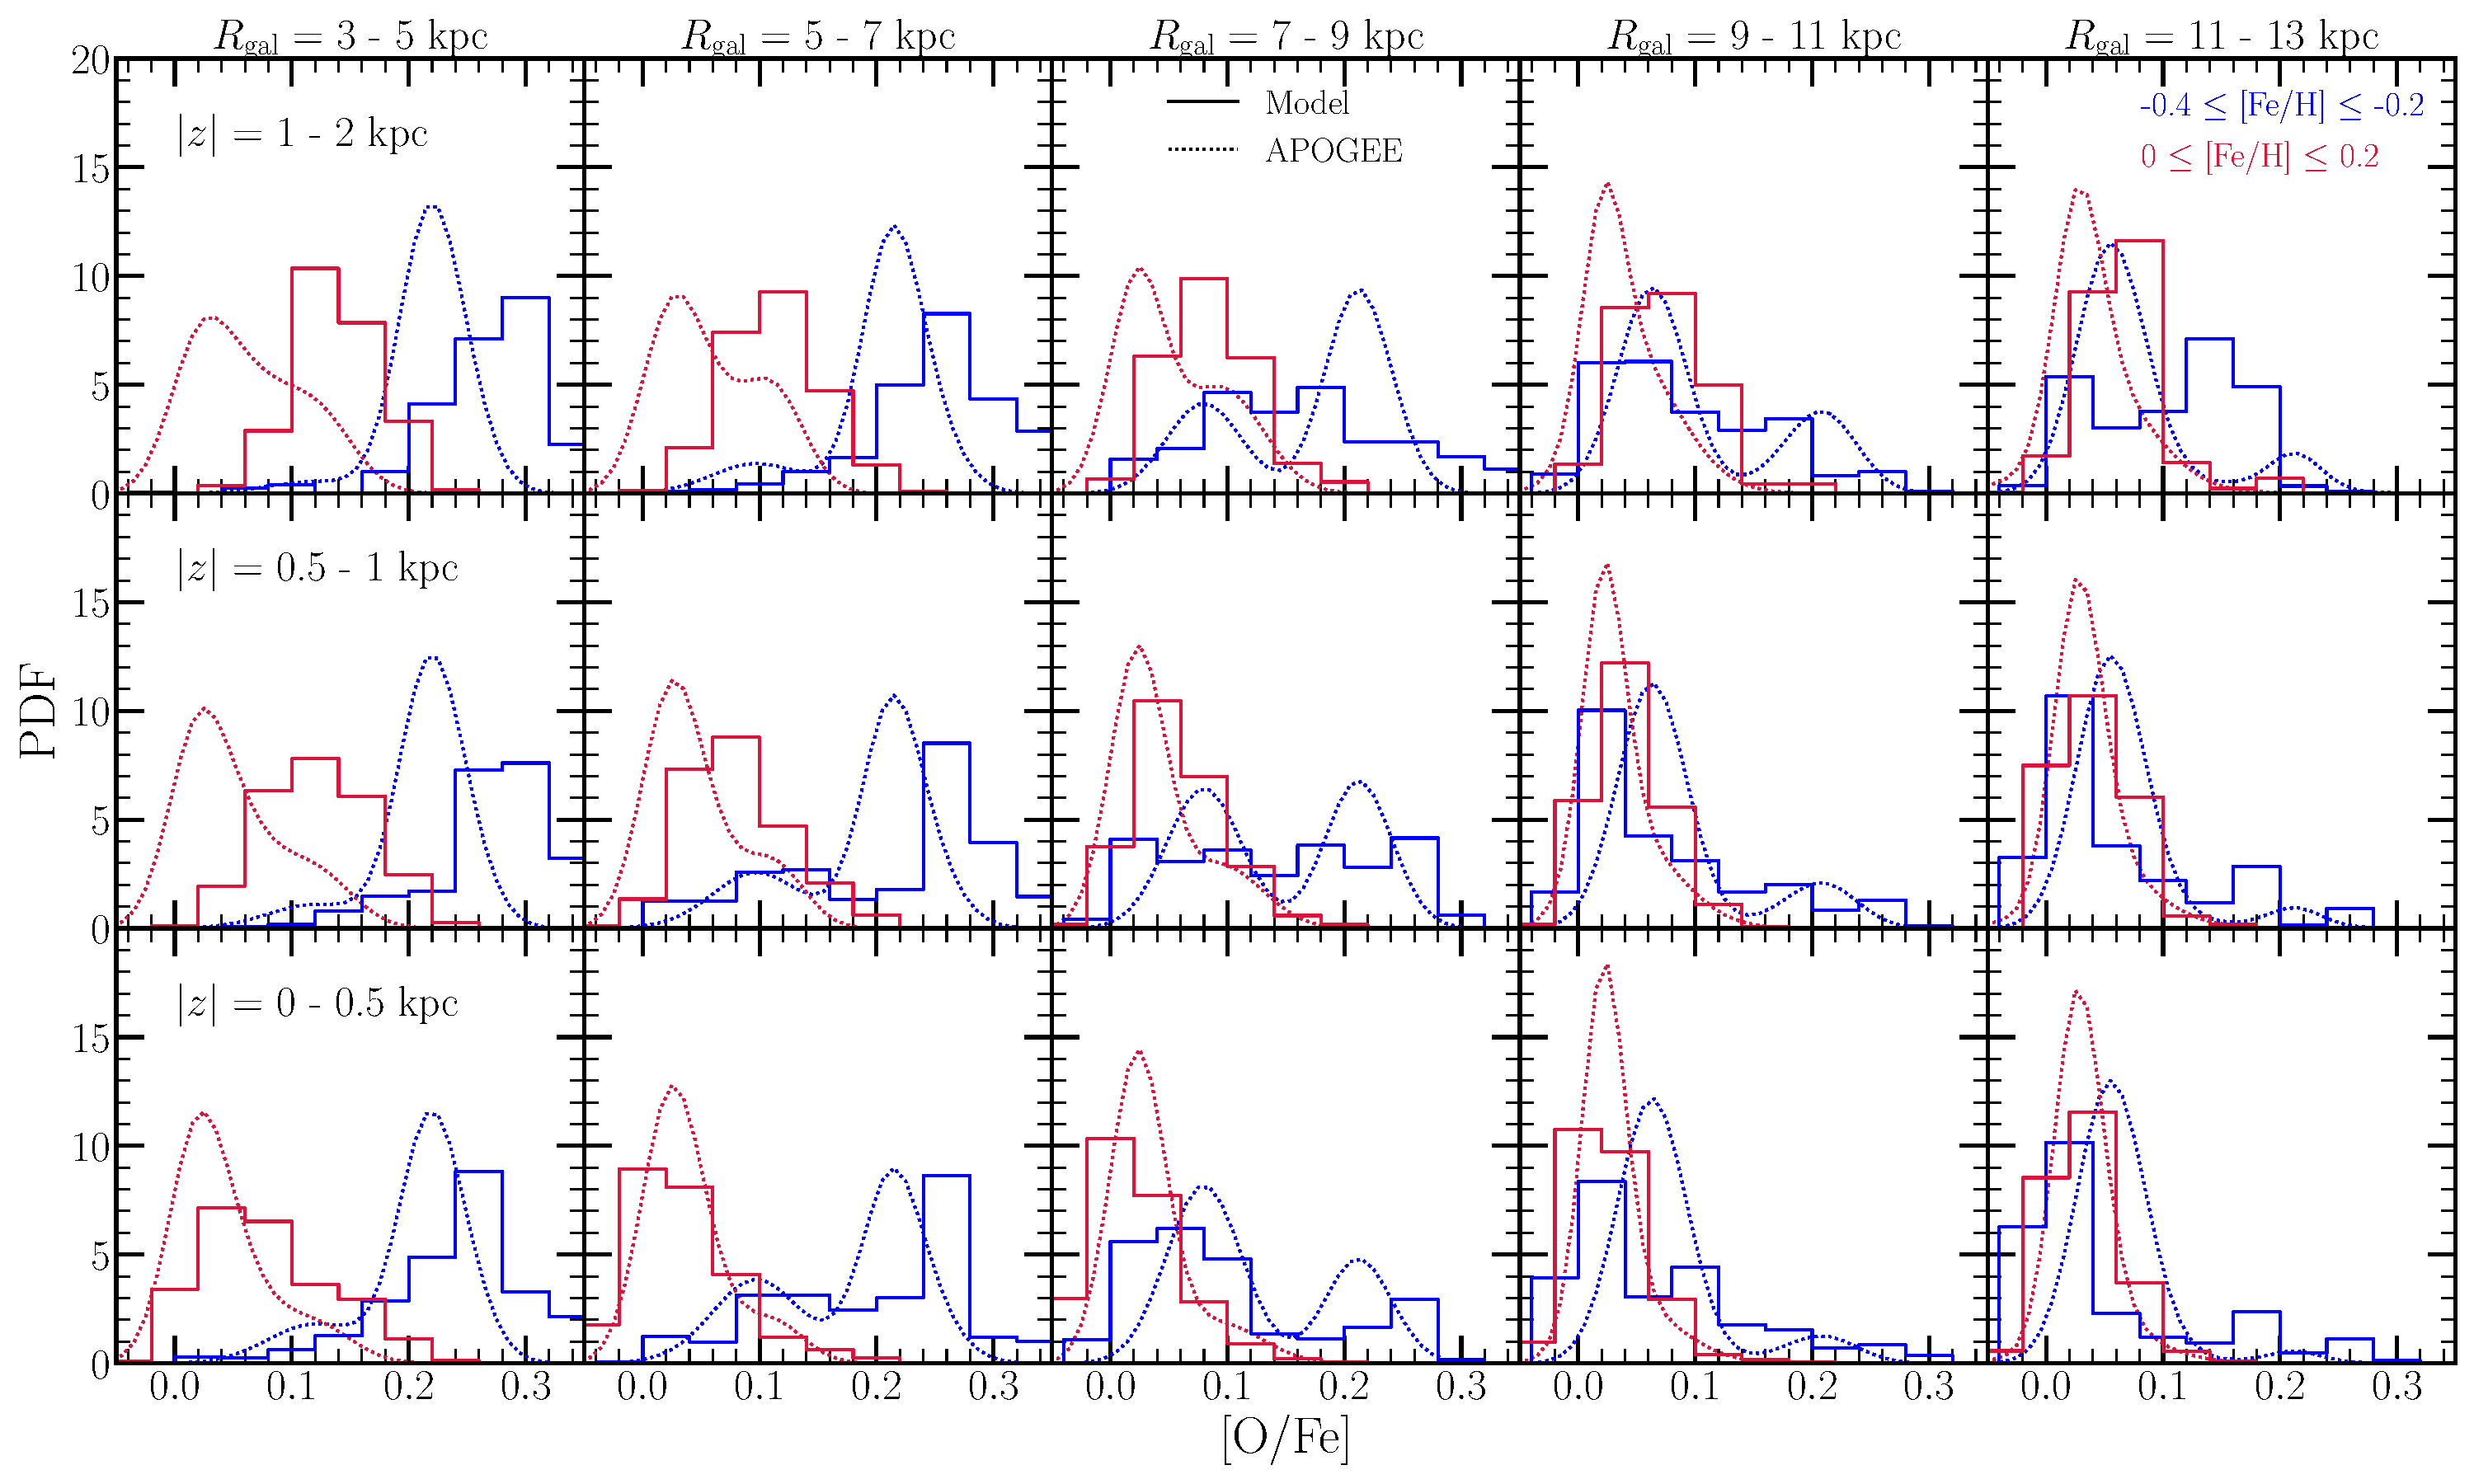
\includegraphics[scale = 0.38]{ofe_mdfs.pdf} 
\caption{Predicted distributions in [O/Fe] in 15 Galactic regions and in two 
bins in [Fe/H]. Columns correspond to bins in~$R_\text{gal}$, denoted at the 
top of each column. Rows correspond to bins in~$\left|z\right|$, denoted in 
text in the left-hand column. Distributions are color-coded according to the 
[Fe/H] the sample is drawn from, denoted by the legend in the upper right 
panel. Solid lines represent that predicted by our inside-out SFH in 
$\Delta$[O/Fe] = 0.04 bins, while dashed lines correspond to the fits to the 
APOGEE DR16 data presented in~\citet{Vincenzo2021a}, which quantify the 
intrinsic distributions accounting for observational uncertainties and the 
APOGEE selection function. } 
\label{migration:fig:ofe_mdfs_insideout} 
\end{figure*} 
\end{landscape}
\clearpage
}

Fig.~\ref{migration:fig:ofe_mdfs_insideout} compares our predicted [O/Fe] distributions 
in Galactic zones to those recently published by 
\citet{Vincenzo2021a}.\footnote{
	\citet{Vincenzo2021a} present [Mg/Fe] distributions in their figures, but 
	they have quantified the [O/Fe] as well, and we use the latter here. 
}
As in our~\S~\ref{migration:sec:obs_comp:mdfs}, they use APOGEE DR16 with similar cuts on 
effective temperature, surface gravity, and signal-to-noise (see their~\S~2). 
They correct for observational scatter as well as age-dependent and (more 
importantly)~\absz-dependent selection in APOGEE to infer the intrinsic 
distribution of [O/Fe] in bins of [Fe/H] that would be found for an unbiased 
sample of long-lived disc stars. 
At a given~\rgal~and [Fe/H],~\citet{Vincenzo2021a} fit a model comprised of two 
Gaussians in [O/Fe], one each for the high-$\alpha$ and low-$\alpha$ 
populations.
The~\absz-dependence of the distribution follows from the empirical scale 
heights of these two populations, taken from~\citet{Bovy2016b}. 
Dotted curves in Fig.~\ref{migration:fig:ofe_mdfs_insideout} show these models integrated 
over the corresponding ranges in~\absz. 
\par 
Solid histograms in Fig.~\ref{migration:fig:ofe_mdfs_insideout} show distributions in 
0.04-dex bins of [O/Fe] for our fiducial inside-out model. 
For clarity we have chosen to focus our comparison on two bins of [Fe/H], one 
just above solar metallicity (0.0~$\leq$ [Fe/H]~$\leq$ 0.2) and one at 
sub-solar metallicity (-0.4~$\leq$ [Fe/H]~$\leq$ -0.2) where the bimodality of 
[O/Fe] is most pronounced. Results for our other models are qualitatively 
similar, and these two [Fe/H] bins illustrate the range of model successes and 
failure. 

% fig 13 
\afterpage{
\clearpage
\begin{landscape}
\begin{figure*} 
\centering 
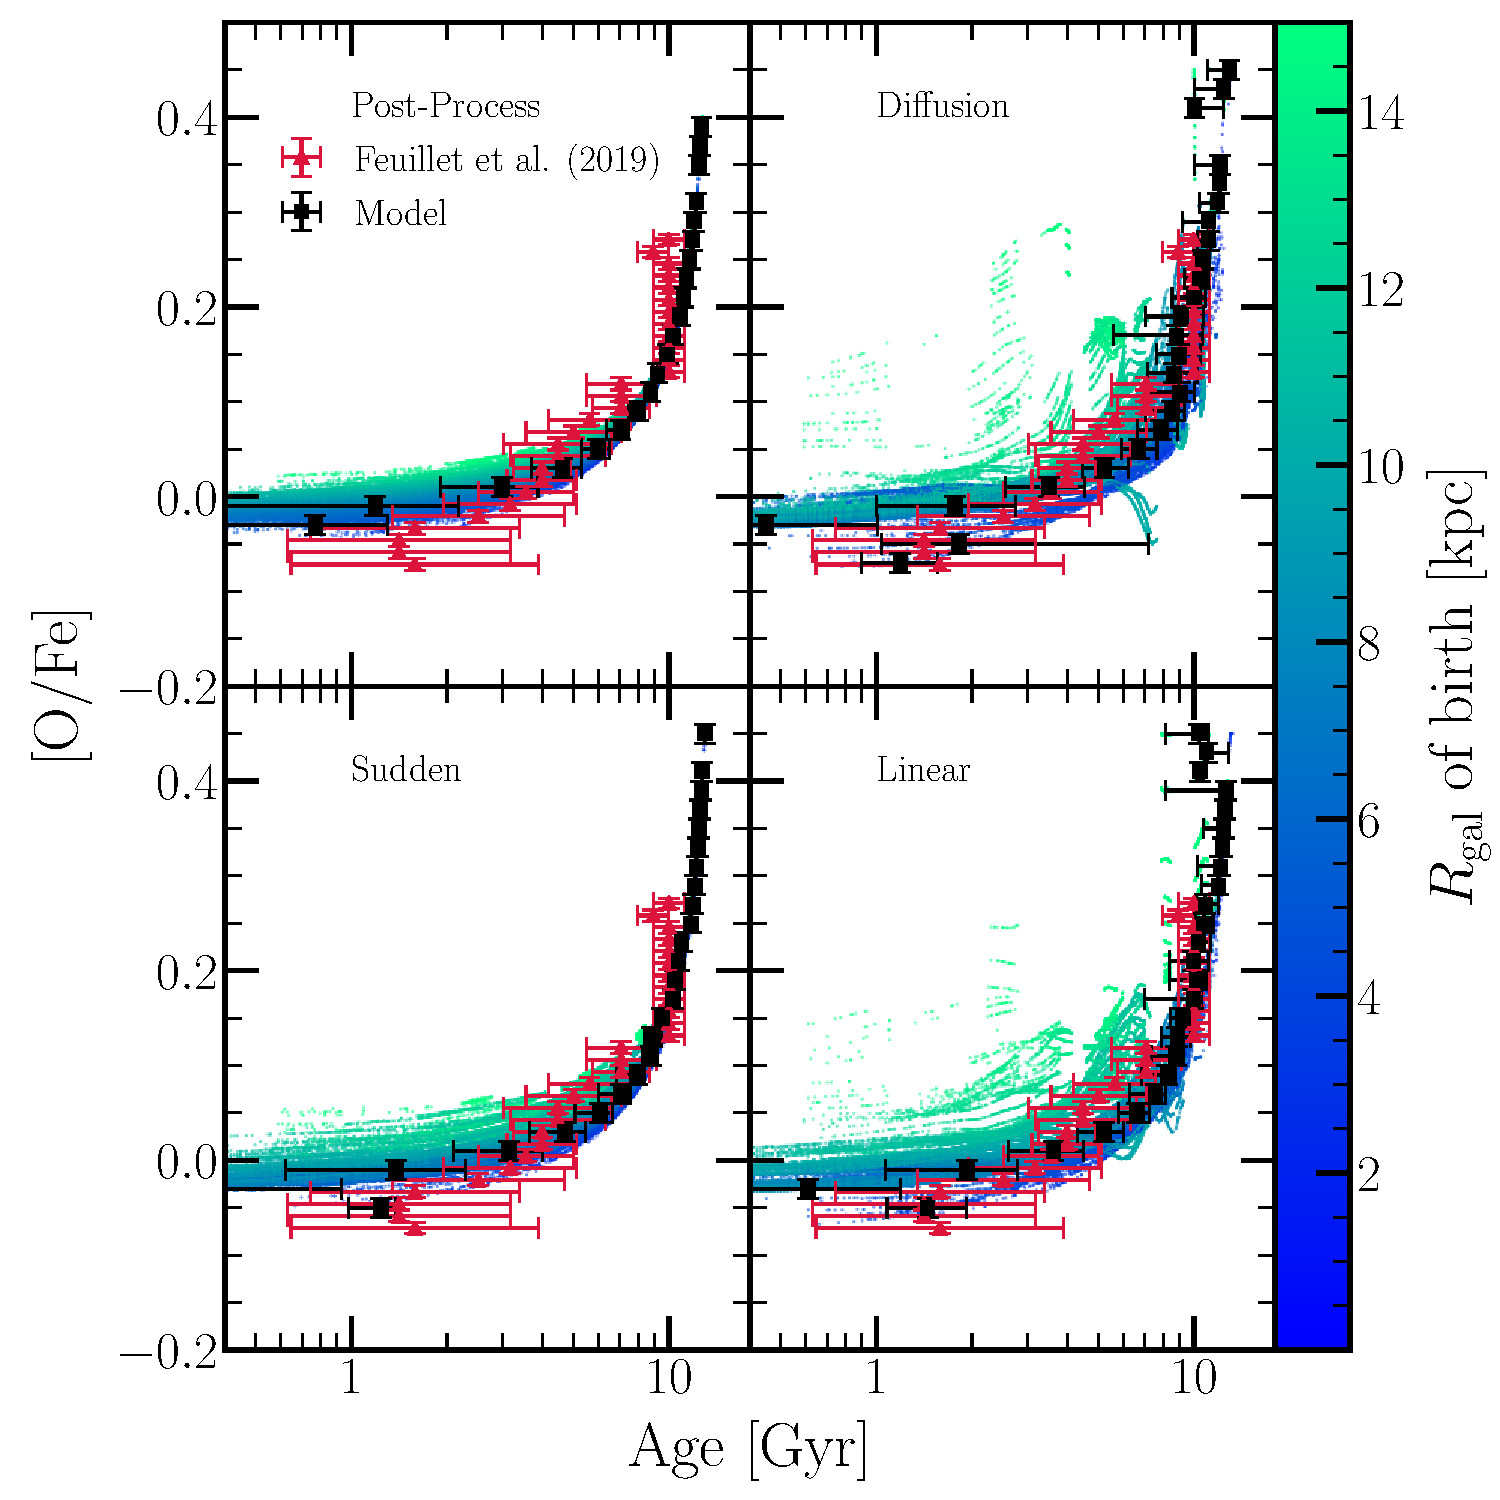
\includegraphics[scale = 0.38]{age_ofe_migration_comparison.pdf} 
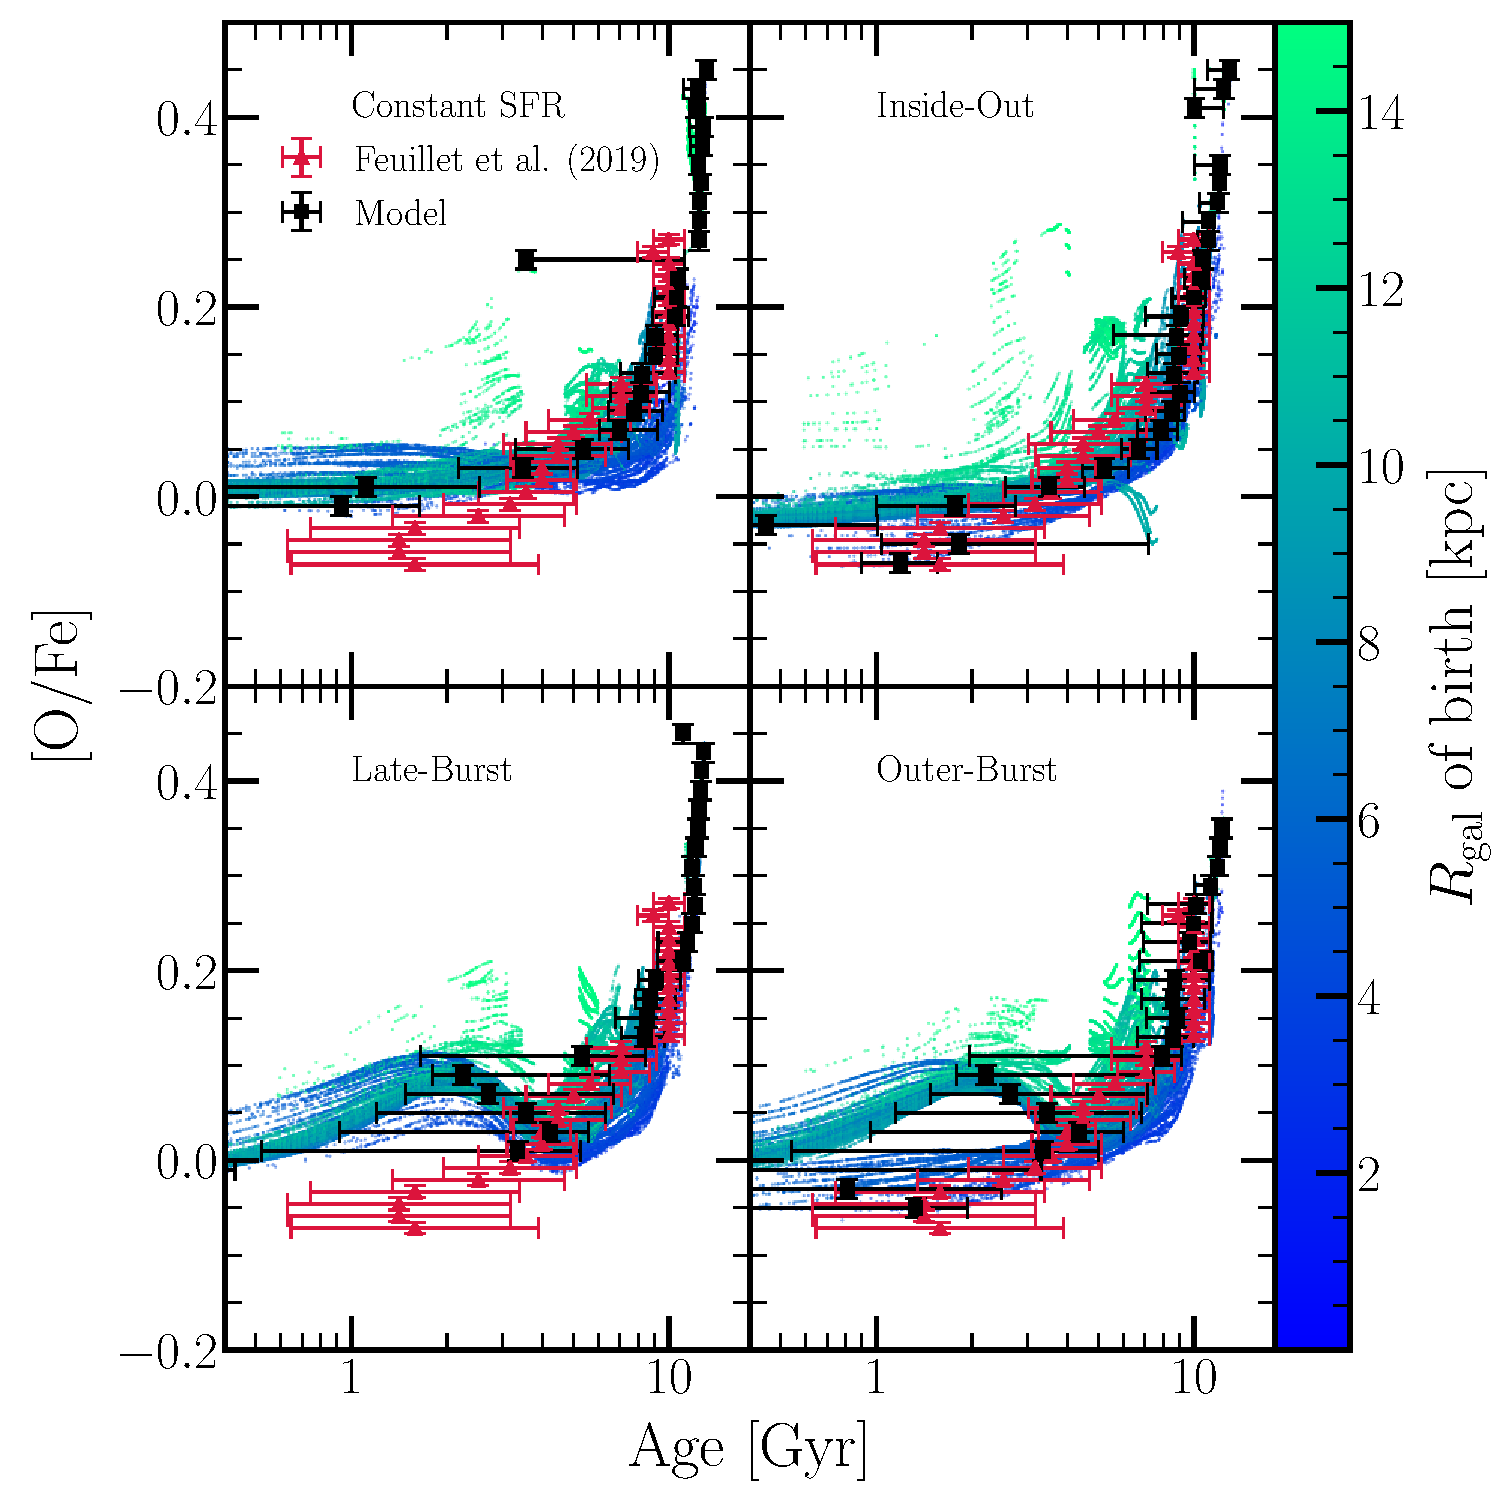
\includegraphics[scale = 0.38]{age_ofe_sfh_comparison.pdf} 
\caption{
\textbf{Left}: A comparison of the predicted age-[O/Fe] relation for the solar 
neighbourhood ($R_\text{gal}$ = 7 - 9 kpc and~$\left|z\right|$ = 0 - 0.5 kpc) 
between the post-processing (upper left), diffusion (upper right), sudden 
(lower left), and linear (lower right) migration models, assuming our 
inside-out SFH. 
\textbf{Right}: The same as the left-hand panels, instead comparing the impact 
of our constant (upper left), inside-out (upper right), late-burst (lower left), 
and outer-burst (lower right) SFHs, assuming diffusion migration. In all panels, 
red triangles and error bars denote the observed median age and dispersion 
thereof in bins of [O/Fe] as reported by~\citet{Feuillet2019}; here we include 
only their bins containing at least 15 stars. Black squares denote the 
mass-weighted median age in 0.02-dex bins in [O/Fe] predicted by our models, 
with error bars denoting the 16th and 84th percentiles of the mass-weighted 
age distribution in those bins. Points in the background denote each individual 
stellar population from the model with a final position in the solar 
neighbourhood, colour-coded according to their Galactocentric radius of birth. 
}
\label{migration:fig:age_alpha} 
\end{figure*} 
\end{landscape}
\clearpage
}

Beginning with the [Fe/H] = 0 - 0.2 bin, we see that the model roughly 
reproduces the observed width of the [O/Fe] distribution. 
In the midplane (\absz~$\leq$ 0.5 kpc) zones it predicts the correct 
skew-positive shape, though the peak of the observed distribution is sharper 
than the model prediction. However, the model histograms shift towards higher 
[O/Fe] with increasing~\absz~while the peak of the observationally inferred 
distributions stays fixed, a discrepancy that is most obvious in the~\rgal~= 
3 - 5 kpc and 5 - 7 kpc bins. The constancy of the observed peak is partly 
a consequence of the~\citet{Vincenzo2021a} fitting procedure, which assumes 
that the location of the high-$\alpha$ and low-$\alpha$ Gaussians stay 
constant at a given~\rgal~and [Fe/H] and only their relative amplitudes change 
with~\absz. We have gone back to the raw data histograms fit by 
\citet{Vincenzo2021a}, and while they do allow some increase in model [O/Fe] 
with~\absz, they do not allow a shift as large as that predicted by our model. 
At~\absz~= 1 - 2 and~\rgal~= 3 - 5 and 5 - 7 kpc, the number of stars 
contributing to the fit is 31 and 17 respectively, so while the shape of the 
distribution is not well constrained, the centroid is robustly determined. 
\par 
This discrepancy could reflect differences in the dynamical heating history 
of the~\hsim~simulation and the Milky Way. 
With its most recent major merger occurring at~$z \approx$ 3, this galaxy was 
previously selected for investigation because of its quiescent merger history 
\citep[e.g.][]{Zolotov2012}. N-body models for the tidal disruption of the 
Sagittarius dwarf galaxy suggest repeated pericentric passages at 1 - 2 Gyr 
intervals~\citep{Law2010}, which could trigger episodes of infall and star 
formation~\citep[e.g.][]{RuizLara2020}. 
These pericentric passages might also heat low-$\alpha$ disc populations to 
higher~\absz, an effect absent in~\hsim. 
Alternatively, we have investigated the impact of changing our~$\eta(\rgal)$ 
prescription to become constant within~\rgal~= 5 kpc, as discussed previously 
in~\S~\ref{migration:sec:obs_comp:mdfs} in the context of the [Fe/H] gradient. 
This change also dampens the predicted trend of [O/Fe] with~\absz~by bringing 
the inner Galaxy's [O/Fe]-[Fe/H] tracks closer together (see 
Figs.~\ref{migration:fig:ofe_feh_diagram} and~\ref{migration:fig:tracks}). 
We find that this change can account for some but not all of the discrepancy, 
shifting the peak of the distribution down by~$\sim$0.05 dex in the upper left 
panel of Fig.~\ref{migration:fig:ofe_mdfs_insideout}. 
\par 
Turning to the -0.4~$\leq$ [Fe/H]~$\leq$ -0.2 bin, the model shows partial but 
by no means complete success. 
It does reproduce the breadth of the [O/Fe] distribution at this intermediate 
metallicity, and in nearly all~\rgal-\absz~zones it predicts skewness of the 
correct sign. 
At~\rgal~= 3 - 5 kpc, the model predicts mode([O/Fe])~$\approx$ 0.3, while 
the observed mode is at [O/Fe]~$\approx$ 0.22. 
This discrepancy is affected by our choice of CCSN yields, which produces an 
[O/Fe] plateau at +0.45. 
While this value is consistent with some observational data (e.g. the 
\citealp*{Ramirez2013} data set modeled by~\citealp{Andrews2017}), APOGEE 
measurements place the plateau at [O/Fe]~$\approx$ +0.3, so it is not 
surprising that our model overpredicts [O/Fe] at low metallicity. 
Unfortunately, uncertainties in the observed abundance scales and the 
theoretical CCSN elemental yields remain an obstacle to sharp GCE model tests. 
\par 
The most significant discrepancy with data is for~\rgal~= 7 - 9 kpc, where the 
observations show a clearly bimodal [O/Fe] distribution in all three~\absz~ 
ranges but the model predicts bimodality only near the midplane. 
This bimodality is also evident in the raw data histograms prior to model 
fitting and correction for selection effects (see Figs. 10 and 11 of 
\citealp{Vincenzo2021a}). 
The idea that radial migration could give rise to an [$\alpha$/Fe] dichotomy 
was proposed by~\citet{Schoenrich2009a}, who noted that the evolutionary tracks 
at any given~\rgal~would produce most stars at low [O/Fe] and that radial 
mixing of these populations would produce a low-$\alpha$ ``sequence'' that is 
a superposition of these evolutionary endpoints. 
\citet{Nidever2014} explored this superposition scenario in the context of 
APOGEE observations, and~\citet{Sharma2021} have recently implemented a 
detailed parameterized scenario matched to APOGEE. 
Although the superposition effect clearly operates in our model, as shown in 
Fig.~\ref{migration:fig:ofe_feh_diagram}, the model produces too many stars at 
intermediate [O/Fe], so there is no clear minimum between the high-$\alpha$ 
and low-$\alpha$ peaks. 
As argued by~\citet{Vincenzo2021a}, the generic problem is that one-zone models 
with smooth evolutionary histories always produce most stars near the low 
[$\alpha$/Fe] endpoints and a much smaller peak at the high-$\alpha$ 
plateau, so one cannot superpose such models in a way that produces strong 
bimodality. 
The~\citet{Sharma2021} model seems like a possible counter-example, but they 
adopt parameterized evolutionary tracks and do not demonstrate that these can 
be drawn from a self-consistent chemical evolution model. 
\par 
The simplest way to produce stronger [$\alpha$/Fe] bimodality in our models 
would be to adopt a two-phase star formation model like that envisioned in 
two-infall scenarios of chemical evolution~\citep[e.g.][]{Chiappini1997, 
Chiappini2001, Romano2010, Grisoni2017, Noguchi2018, Palla2020, Spitoni2016, 
Spitoni2018, Spitoni2019, Spitoni2020, Spitoni2021}. 
% {\color{red} 
\citet{Mackereth2018} find similar conclusions in a sample of 133 Milky 
Way-like galaxies from the EAGLE simulation.
% } 
These scenarios turn down the SFR while the ISM abundances pass through the 
intermediate [$\alpha$/Fe] regime. 
Other scenarios such as large early starbursts~\citep{Clarke2019} or reverse 
[Fe/H] evolution with late-time outflows~\citep{Weinberg2017b} could also 
enhance bimodality, but the late starbursts considered here are insufficient 
on their own. 
We will explore these alternative scenarios for the origin of bimodality in 
future work. 

\subsection{The Age-[$\alpha$/Fe] Relation} 
\label{migration:sec:obs_comp:age_alpha} 

% fig 14 
\afterpage{
\clearpage
\begin{landscape}
\begin{figure*} 
\centering 
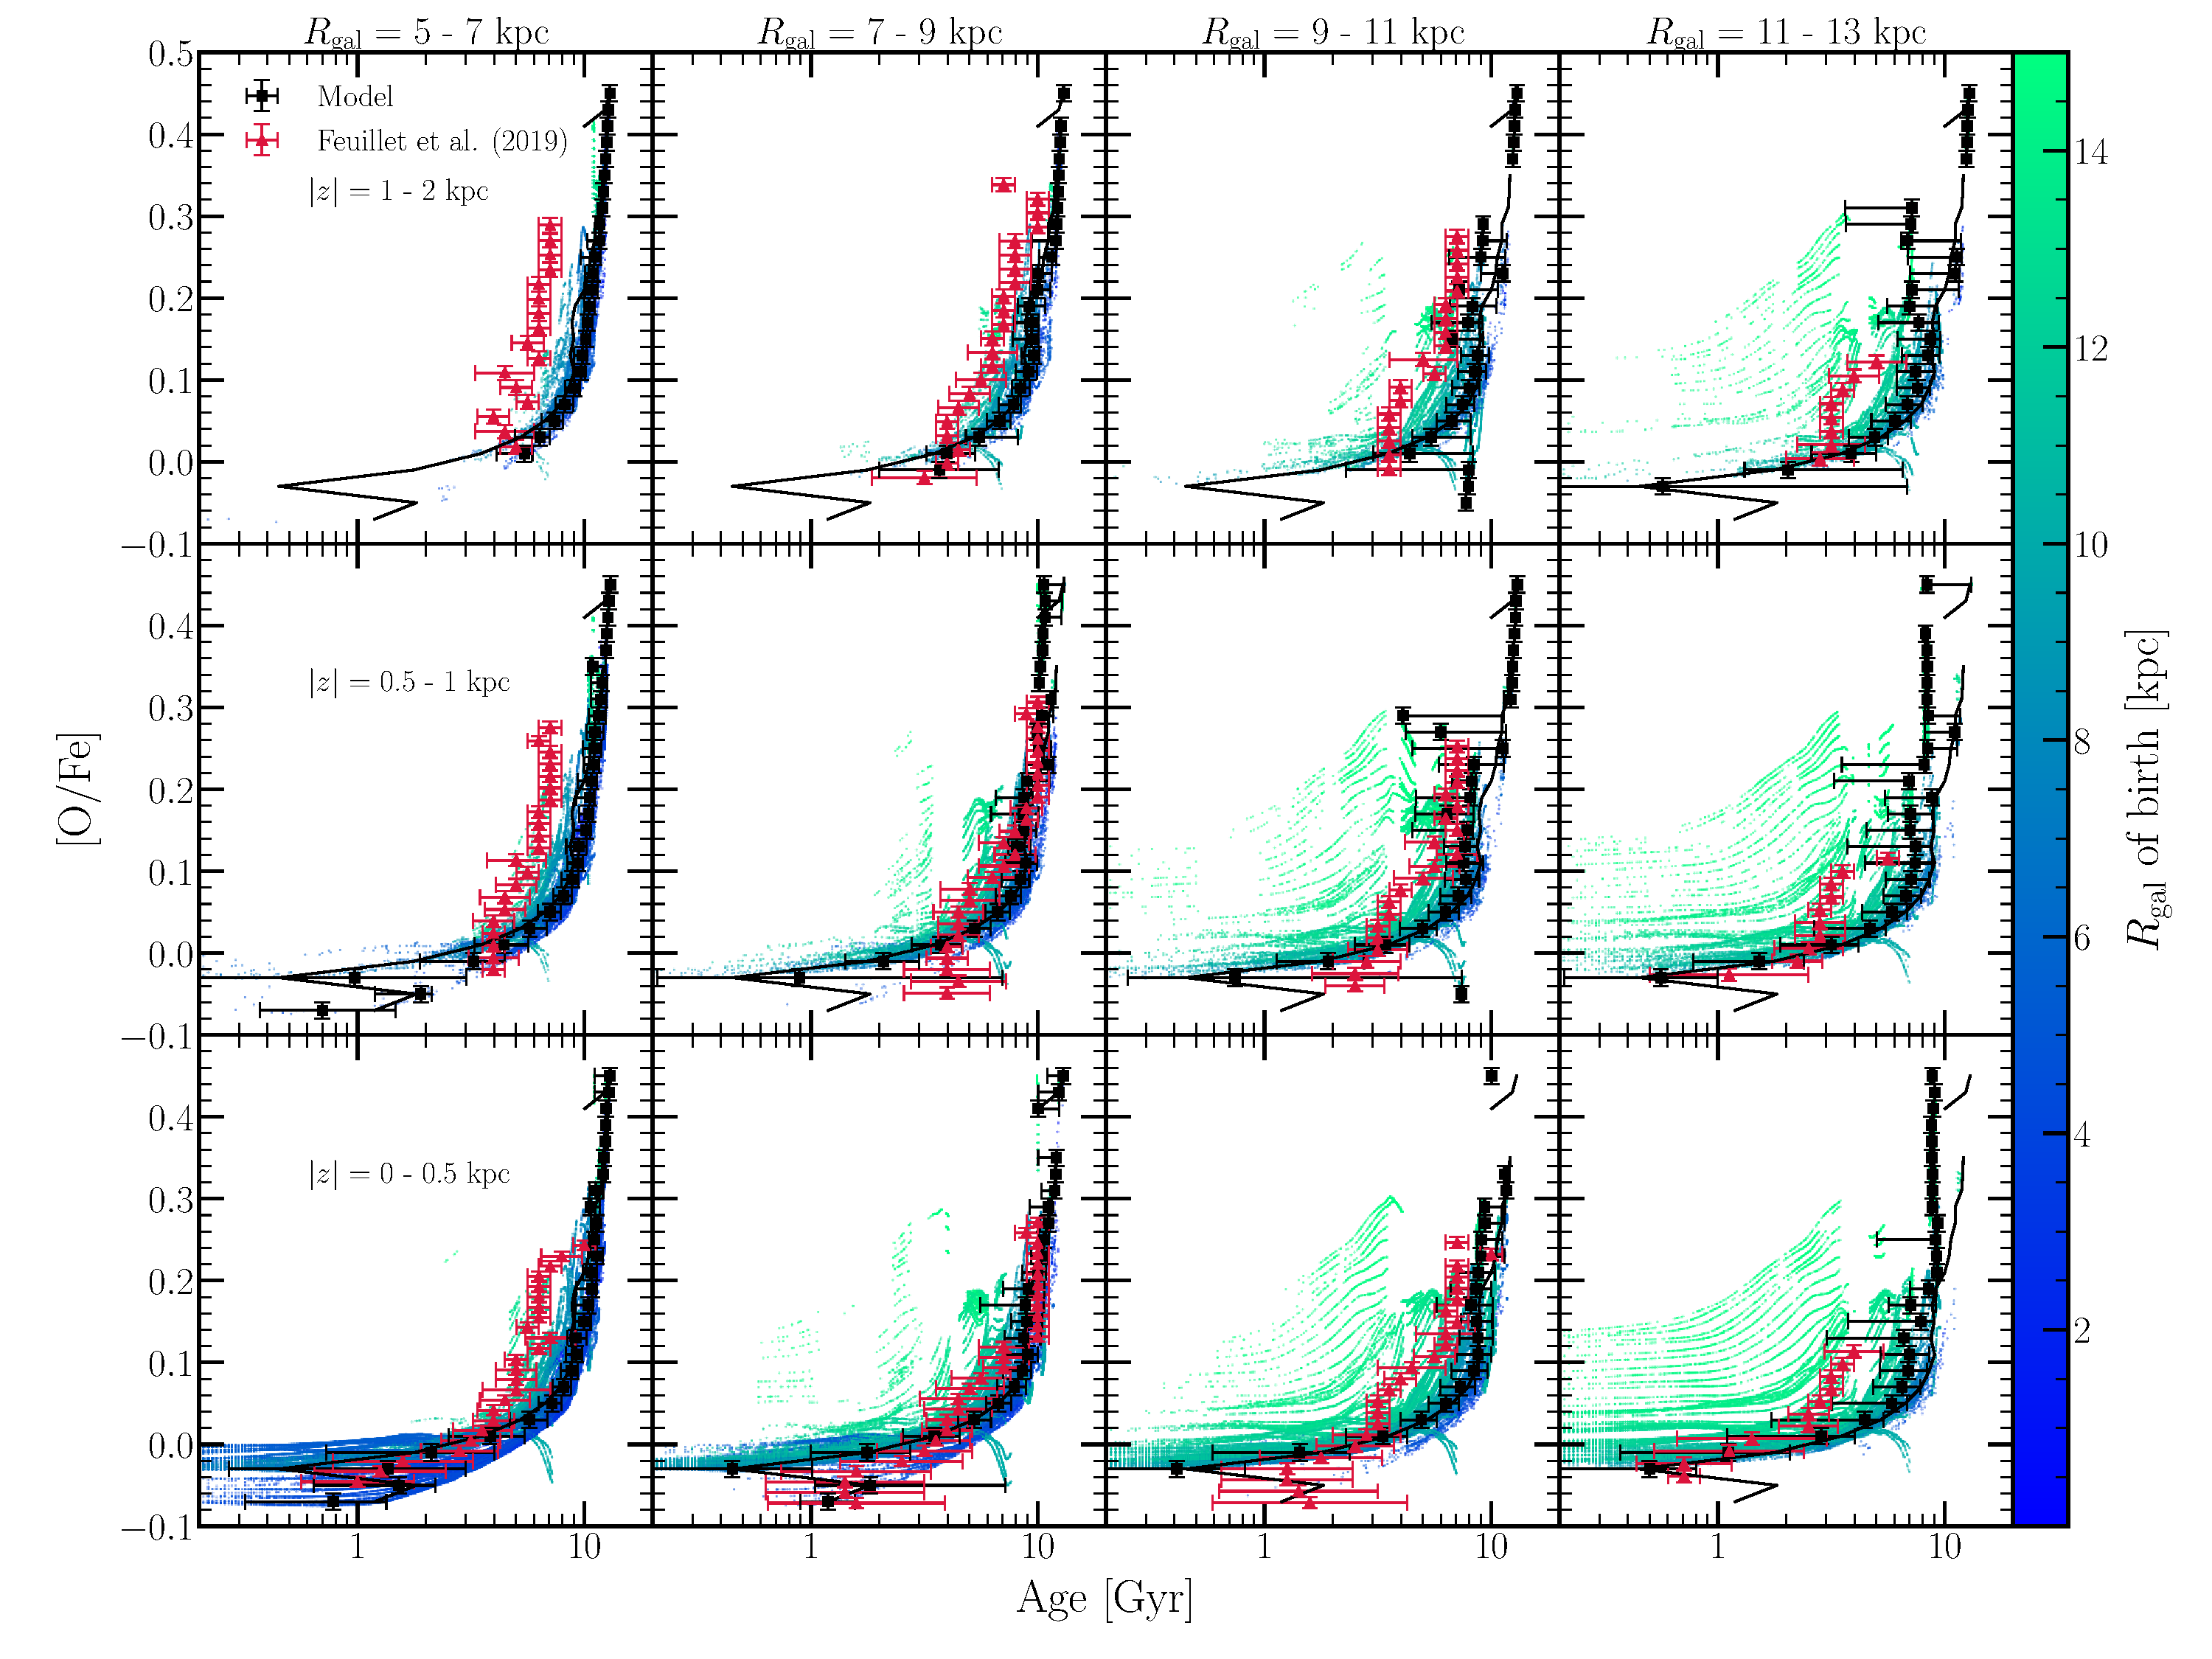
\includegraphics[scale = 0.35]{age_alpha_regions.pdf} 
\caption{The age-[O/Fe] relation in 12 Galactic regions predicted by our 
inside-out SFH. Bins in Galactocentric radius are shown in columns, and labeled 
at the top. 
Bins in the disc midplane distance~\absz~are shown in rows, noted in the 
left-hand column. Red triangles, black squares, 
error bars, and background points are as in Fig.~\ref{migration:fig:age_alpha} for the 
corresponding Galactic region. The solid black line connects the black squares 
in the bottom, left-middle panel, and is replicated elsewhere for reference. } 
\label{migration:fig:age_alpha_regions} 
\end{figure*} 
\end{landscape}
\clearpage
}

In this section, we assess the predicted age-[O/Fe] relations of our models, 
using the results of~\citet{Feuillet2019} as the observational benchmark. 
Their stellar age measurements are based on isochrone matching, 
using APOGEE DR14 stars for which parallax measurements are available 
from~\gaia~\citep{Abolfathi2018, GaiaCollaboration2018}.
With their spatial and quality cuts, the final sample consisted of 77,562 
stars. 
In bins of [O/Fe], they assume a Gaussian distribution of log age, fitting the 
mean (or equivalently, the median) and standard deviation to the stars in that 
bin. 
The choice of a Gaussian distribution is driven by simplicity, enabling 
estimates of mean and spread for data with significant age errors, but because 
our model predicts non-Gaussian log age distributions at fixed [O/Fe], the 
comparison to data is not free of nuance. 
We base most of our model comparisons below on the mass-weighted median age, 
simply denoting the 50th percentile of the mass-weighted age distribution of 
some subsample. 
\par 
In the left-hand set of panels of Fig.~\ref{migration:fig:age_alpha}, we compare the 
age-[O/Fe] relation in the solar neighbourhood ($R_\text{gal}$~= 7 - 9 kpc and 
$\left|z\right|\leq$~0.5 kpc)\footnote{
	In order to avoid confusion, we distinguish between solar ``annulus'' and 
	solar ``neighbourhood'' by defining the solar neighbourhood to be the 
	solar annulus population at~\absz~$\leq$~0.5 kpc. This definition should 
	approximate a sample within a spherical radius of~$\sim$0.5 kpc around the 
	Sun, similar to typical observational definitions. 
} predicted by our four migration models to the 
\citet{Feuillet2019} measurements, shown in red triangles. 
We mark the mass-weighted median age in bins of [O/Fe] in each model with black 
squares, and plot for reference in the background each individual stellar 
population in the solar neighbourhood, colour-coded according to its 
Galactocentric radius of birth. 
\par 
The median age-[O/Fe] trend is similar for all four migration prescriptions, 
and the model prediction is in reasonable agreement with the APOGEE 
measurements. 
From the colour-coding in the post-processing model, one can see that the 
predicted relation is insensitive to the chemical evolution parameters across 
the range represented in our Galactic radial zones, differing only in the 
precise value of [O/Fe] reached at late times. 
Nonetheless, these differences are large enough that radial mixing causes a 
large spread in age at low values of [O/Fe], where the median trend itself 
becomes shallow. 
Nearly all high [O/Fe] stars are old. 
The spread is similar, but not identical, among the four migration 
prescriptions, and it is in reasonable agreement with the observationally 
inferred spread. 
This agreement is a significant success of the migration predicted by the
\hsim~simulation in concert with our GCE model. 
% The observed [O/Fe] distribution extends to values below -0.05 that are not 
% present in our model. This difference could reflect missing stochasticity in 
% our model, or slightly incorrect yield or SFH choices, or observational errors 
% in some [O/Fe] measurements. 
\par 
Although their median trends and characteristic spreads are similar, the 
diffusion and linear migration models show a marked diffrence from the 
post-processing and sudden models, predicting populations of young 
($\lesssim$ 4 Gyr) and intermediate age (4 - 7 Gyr)~$\alpha$-enhanced stars 
([O/Fe]~$\approx$ +0.1 - 0.2) in the solar neighbourhood, which formed at large 
\rgal~with [O/Fe] values well above the main trend for their age. 
They arise from the large fluctuations in the SN Ia rate at large~\rgal~shown 
in Fig.~\ref{migration:fig:tracks} and discussed in~\S~\ref{migration:sec:obs_comp:gradient}, 
which occur when stellar populations migrate to different radii before 
producing most of their SNe Ia. 
% When the SN Ia Fe production rate fluctuates downward, [O/Fe] fluctuates 
% upward in the ISM, and the stars that form from it inherit such a composition. 
% These stars then migrate to the solar annulus. 
% These stars can then migrate to the solar annulus. 
% {\color{red} 
SNe Ia account for~$\sim$60\% of the Fe production at all metallicities 
in our models (see discussion in~\S~\ref{migration:sec:methods:yields}). 
Visual inspection of Fig.~\ref{migration:fig:tracks} indicates that the SN Ia rate can 
vary by as much as a factor of~$\sim$3 at~$\rgal\gtrsim$~9 kpc in our models, 
sometimes more in extreme cases, simply because their progenitors are 
migrating; this corresponds to variability as large as~$\sim$40\% in the total 
Fe enrichment rate if everything else is constant. 
This variability can arise in part out of efficient radial migration moving 
stars away from their birth radii faster than the SN Ia timescale as well as 
the combination of the long tail of the SN Ia DTD and migration on longer 
timescales (see discussion at the end of~\S~\ref{migration:sec:methods:h277}). 
The [$\alpha$/Fe] ratio at a given time is approximately determined by the 
ratio of core collapse to type Ia supernova events occurring over the previous 
depletion time~\citep{Weinberg2017b}, which can be short in the outer Galaxy in 
our models due to the substantial outflows at these radii (see discussion 
in~\S~\ref{migration:sec:methods:outflows}). 
Consequently, when the SN Ia Fe production rate fluctuates downward, [O/Fe] 
fluctuates upward in the ISM. 
An alternative explanation for young~$\alpha$-rich stars is a burst of 
star formation, when the ISM becomes~$\alpha$-enhanced because the CCSN rate 
increases~\citep{Johnson2020}. 
The explanation suggested here is in some sense the opposite: the ISM 
becomes not necessarily~$\alpha$-rich but Fe-poor because of fewer SNe Ia. 
The stars that form inherit such a composition and can then migrate to 
the solar annulus, and our models predict the variability to be sufficiently 
large to explain the high [$\alpha$/Fe] ratios seen in APOGEE. 
% }
% \par\null\par 
\par
The presence of young and intermediate-age~$\alpha$-enhanced stars in APOGEE 
has been demonstrated using ages based on carbon-to-nitrogen ratios 
\citep{Martig2016} calibrated against the asteroseismic ages of the APOKASC 
catalog~\citep{Pinsonneault2014}, and with the asteroseismic ages directly 
\citep{Martig2015, Jofre2016, Izzard2018, SilvaAguirre2018}. 
% \par 
\citet{SilvaAguirre2018} demonstrate that these stars have kinematics similar 
to the rest of the high-$\alpha$ population, and they suggest that they are 
in fact old stars ``rejuvenated'' by mergers or mass transfer events 
% {\color{red} 
as postulated by~\citet{Jofre2016} and~\citet{Izzard2018}. 
In a sample of four young~$\alpha$-enhanced stars observed with Gemini-GRACES, 
\citet{Yong2016} find that two (possibly three) of them show evidence of a 
debris disc, indicative of previous interactions with a binary companion. 
% } 
In a sample of 51 young,~$\alpha$-rich red giants,~\citet{Hekker2019} 
demonstrate that a portion of these stars have carbon-to-nitrogen ratios 
consistent with mass transfer events, but that others do not, indicating that 
they are either truly young stars or the result of mergers on the main 
sequence. 
% \citet{Weinberg2017b} and~\citet{Johnson2020} proposed that
% young~$\alpha$-rich stars could arise in bursts of star formation that 
% enhance the rate of CCSN enrichment. 
% The explanation suggested here is in some sense the opposite: the 
% stars are not so much~$\alpha$-rich as they are Fe-poor because of the 
% deficit in SNe Ia events. 
% {\color{red} 
Our model does not refute mass transfer as an origin for some massive, 
$\alpha$-rich stars, but it can explain the truly young, intrinsically 
$\alpha$-enhanced stars which appear to make up a portion of the 
young~$\alpha$-rich population separate from those which formed via mass 
transfer~\citep{Yong2016, Hekker2019}. 
% }
In our diffusion model,~$\sim$0.2\% of solar neighbourhood stars with 0.1~$\leq$ 
[O/Fe]~$\leq$ 0.2 have ages below 4 Gyr, but~$\sim$13.9\% have ages below 7 Gyr. 
% {\color{red} 
They have a broad distribution in metallicity spanning from [Fe/H]~$\approx-1$ 
to~$\sim$solar, with multiple peaks indicative of separate sub-populations. 
This large spread qualitatively agrees with the findings 
of~\citet{SilvaAguirre2018} (see their Figs. 8 and 10) and~\citet{Miglio2021} 
(see their Fig. 5). 
A direct comparison to data is not free of nuance, because the 
young~$\alpha$-rich stars which formed via mass transfer may outnumber 
those which are intrinsically young~\citep{Miglio2021}. 
% } 

% fig 15 
\begin{figure} 
\centering 
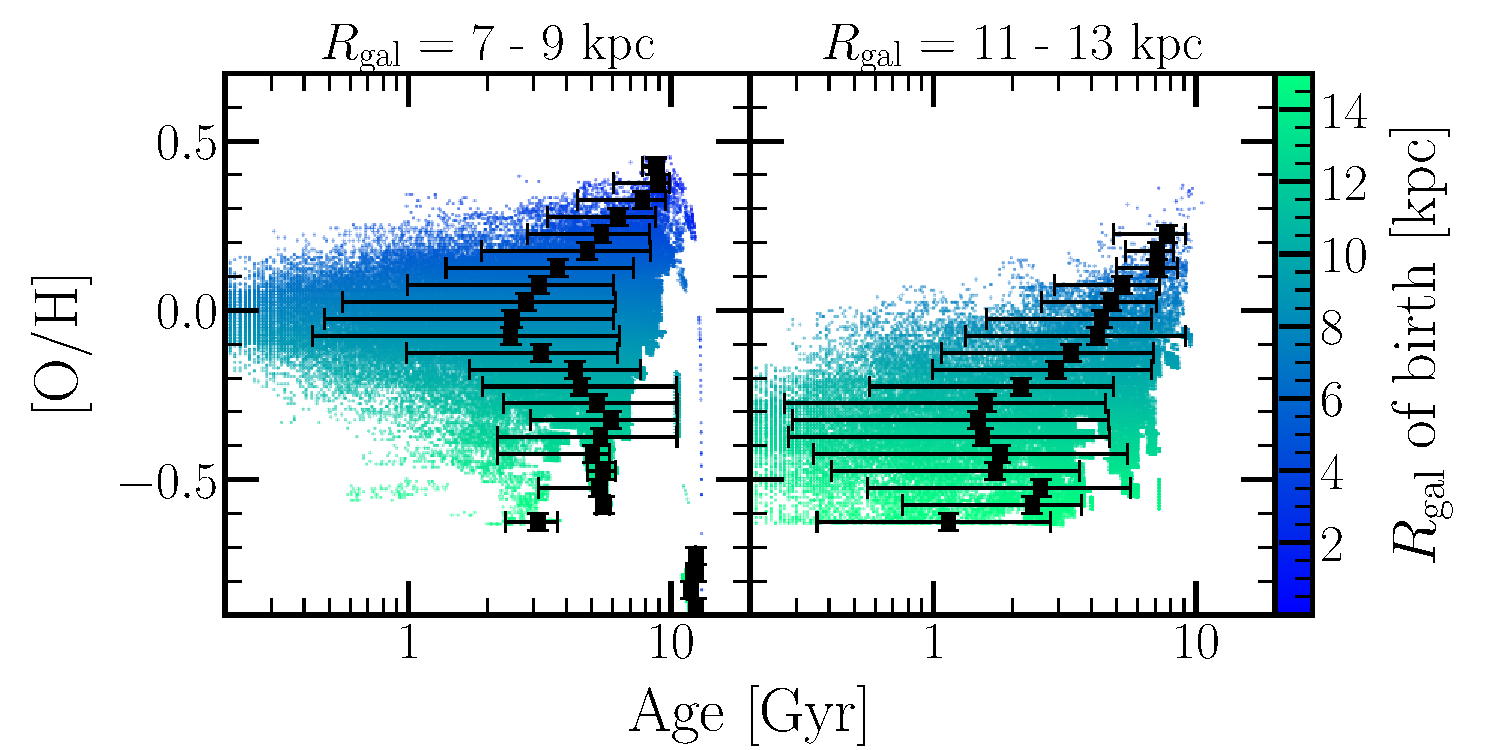
\includegraphics[scale = 0.45]{amr_static_o.pdf} 
\caption{The age-[O/H] relation predicted by our constant SFR model for 
$R_\text{gal}$~= 7 - 9 kpc (left) and 11 - 13 kpc (right). Each panel plots 
only the~$\left|z\right|\leq$~0.5 kpc population. The colored points in the 
background and the black squares with error bars are as in Fig. 
\ref{migration:fig:age_alpha}, but with the model prediction quantified in bins 
of~$\Delta$[O/H] = 0.05. } 
\label{migration:fig:age_oh_static} 
\end{figure} 

The right panels of Fig.~\ref{migration:fig:age_alpha} compare the model predictions of 
our four different SFHs, all assuming the diffusion migration prescription, 
with the same plotting scheme and colour-coding as in the left panels. 
The predicted trend for the constant SFR model is similar to that of the 
inside-out model, but the agreement with data is slightly worse because with a 
constant SFR the evolutionary tracks do not extend below solar [O/Fe]. 
The starburst models, on the other hand, predict a 0.05 - 0.1 dex upward 
fluctuation in [O/Fe] at ages of 1 - 3 Gyr due to the perturbed ratio of 
core-collapse to Type Ia supernova rates~\citep{Johnson2020}. 
In the outer-burst model, stars formed at~\rgal~> 6 kpc follow this perturbed 
track while stars from the inner Galaxy follow the original track. 
These models are motivated by observational results which provide empirical 
evidence for elevated recent star formation~\citep{Mor2019, Isern2019}. 
However, in conjunction with our chemical evolution prescriptions they produce 
clear disagreement with the age-[O/Fe] distributions of~\citet{Feuillet2019} 
and~\citet{Miglio2021}. 
This disagreement could indicate that the starbursts were more limited in 
Galactic radius than we have assumed, or that some other ingredient is missing 
from our models. 
The discrepancy in these panels also implies that if young~$\alpha$-rich stars 
do arise in a starburst, then it must remain sufficiently localized that the 
resultant stellar populations remain outliers from an otherwise monotonic 
age-[$\alpha$/Fe] relation. 
\par 
Fig.~\ref{migration:fig:age_alpha_regions} extends the comparison of our baseline, 
inside-out model and the observations of~\citet{Feuillet2019} to other 
Galactic regions. 
The predicted median age-[O/Fe] trend is nearly independent of location, as we 
can see by comparing the black model points in each panel to the black line, 
which shows the solar neighbourhood prediction. 
~\citet{Feuillet2019} report ages for~$\alpha$-rich stars that are younger at 
large~$R_\text{gal}$ and high $\left|z\right|$, though in most cases only by 
$\sim$20\%. 
Our model predicts a larger population of intermediate-age~$\alpha$-rich stars 
at large~\rgal, but this effect is not large enough to reproduce the observed 
trend. 
None of our model variants reproduce this trend of age-[O/Fe] offset with~\absz, 
so if the observational result is correct then it points to a missing 
ingredient in the model. 
As with the overpredicted [O/Fe] ratios at 
small~\rgal~(\S~\ref{migration:sec:obs_comp:ofe_dists}), dynamical stirring of younger 
disc populations to higher~\absz~by the Sagittarius dwarf could play a role in 
resolving this discrepancy. 
However, Fig.~\ref{migration:fig:age_alpha_regions} shows that the model does not have a 
reservoir of younger high-$\alpha$ stars at low-\absz~available to be stirred, 
so some additional change would likely be needed. 
Furthermore, our model predicts the 16th-84th percentile ranges of the age 
distribution at fixed [O/Fe] to increase for [O/Fe]~$\gtrsim$ +0.1 stars, at 
least in part due to the higher frequency of young and intermediate-age 
$\alpha$-rich stars. 
This increase in the intrinsic scatter of the relation is simply a consequence 
of the SN Ia rate variability having a higher amplitude at large~\rgal~(see 
discussion in~\S~\ref{migration:sec:obs_comp:gradient}). 
\par 
In this paper, Fe is the only element that we consider with a delayed 
nucleosynthetic source. 
Nonetheless, we expect stellar migration to induce similar variability and 
scatter for other elements with delayed sources. 
Elements such as strontium (Sr) are produced by the $s$-process in AGB stars on 
a timescale intermediate between CCSN and SN Ia enrichment (see Fig. 5 of 
\citealp{Johnson2020}), and elements with a large contribution from low mass 
AGB stars could trace longer timescales. 
The DTD for $r$-process elements such as europium (Eu) is uncertain because the 
relative importance of prompt sources (e.g., collapsars) and delayed sources 
(e.g., neutron star mergers) remains poorly constrained~\citep{Cote2019, 
Mishenina2019, Siegel2019, Vincenzo2021b}. 
Using hydrodynamical simulations from the Auriga project~\citep{Grand2017}, 
\citet{vandeVoort2020} indeed find that the intrinsic scatter in $r$-process 
abundances increases for models with longer characteristic delay times. 
Future comparisons of observed trends between age and abundance ratios with the 
predictions of models like those presented here could better isolate missing 
ingredients of the models, as well as potentially improving understanding of 
the nucleosynthetic sources. 
% \par 
% {\color{red} (The next paragraph probably moving to conclusions) I added a 
% couple sentences to the prior paragraph that, with what is currently stated in 
% the conclusions, may make this redundant. -James}  
% In our models, radial mixing of populations with different evolutionary tracks 
% is the only effect that creates a spread of abundance ([Fe/H] and [O/Fe]) at 
% fixed age at a given final~\rgal. 
% The trend of evolutionary tracks with birth radius is fairly smooth, though 
% the impact of migration on SN Ia rates creates stochastic variations that 
% give rise to the young and intermediate-age~$\alpha$-rich stars in our models. 
% Incomplete mixing of the ISM in azimuth and~\absz~\citep{Krumholz2018b} is an 
% additional source of stochasticity in chemical evolution that is currently not 
% represented in our models. 
% This stochasticity will be larger for elements produced by rare events, such as 
% neutron star mergers, and there have been some recent theoretical 
% investigations of predicted scatter in~$r$-process abundances from this source 
% \citep[e.g.][]{vandeVoort2020}. 
% Observationally, the correlation of residual abundances (i.e., of deviations 
% from mean trends) may be a more sensitive probe of stochasticity and mixing 
% than variance of abundance ratios~\citep{Ting2021}. Characterizing the physics 
% of element mixing in the ISM and the stochastic effects on chemical evolution 
% is an important frontier for models and observations. 

\subsection{The Age-Metallicity Relation} 
\label{migration:sec:obs_comp:amr} 

% fig 16 
\begin{figure} 
\centering 
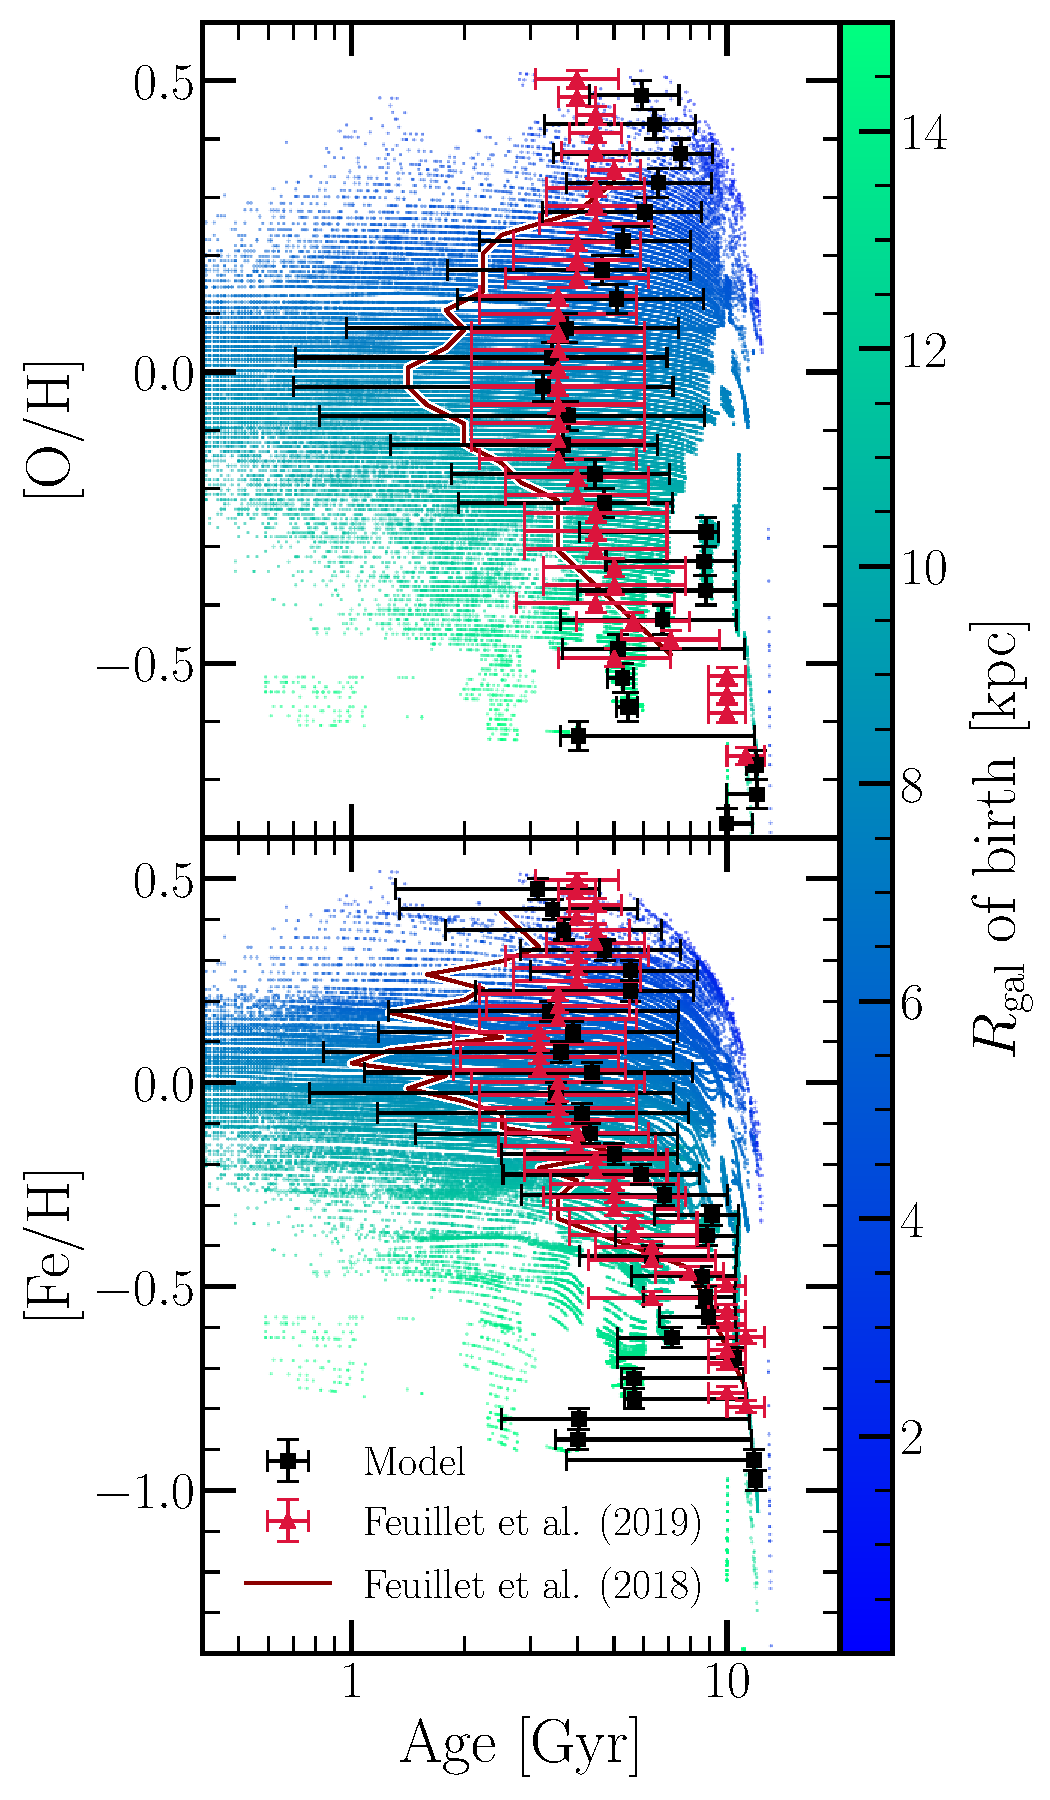
\includegraphics[scale = 0.5]{amr_solar_annulus.pdf} 
\caption{The age-[O/H] (top) and age-[Fe/H] (bottom) relations for the solar 
neighbourhood (i.e.~$R_\text{gal}$ = 7 - 9 kpc,~$\left|z\right|\leq$~0.5 kpc) 
as predicted by the fiducial model. Red triangles, black squares, error bars, 
and background points are as in Fig.~\ref{migration:fig:age_alpha}, but with the model 
prediction quantified in bins of~$\Delta$[O/H] =~$\Delta$[Fe/H] = 0.05. For 
comparison, we plot the~\citet{Feuillet2018} measurements in a dark red line, 
omitting the associated uncertainties for visual clarity. } 
\label{migration:fig:amr_solar_annulus} 
\end{figure} 

% fig 17 
\afterpage{
\clearpage
\begin{landscape}
\begin{figure*} 
\centering 
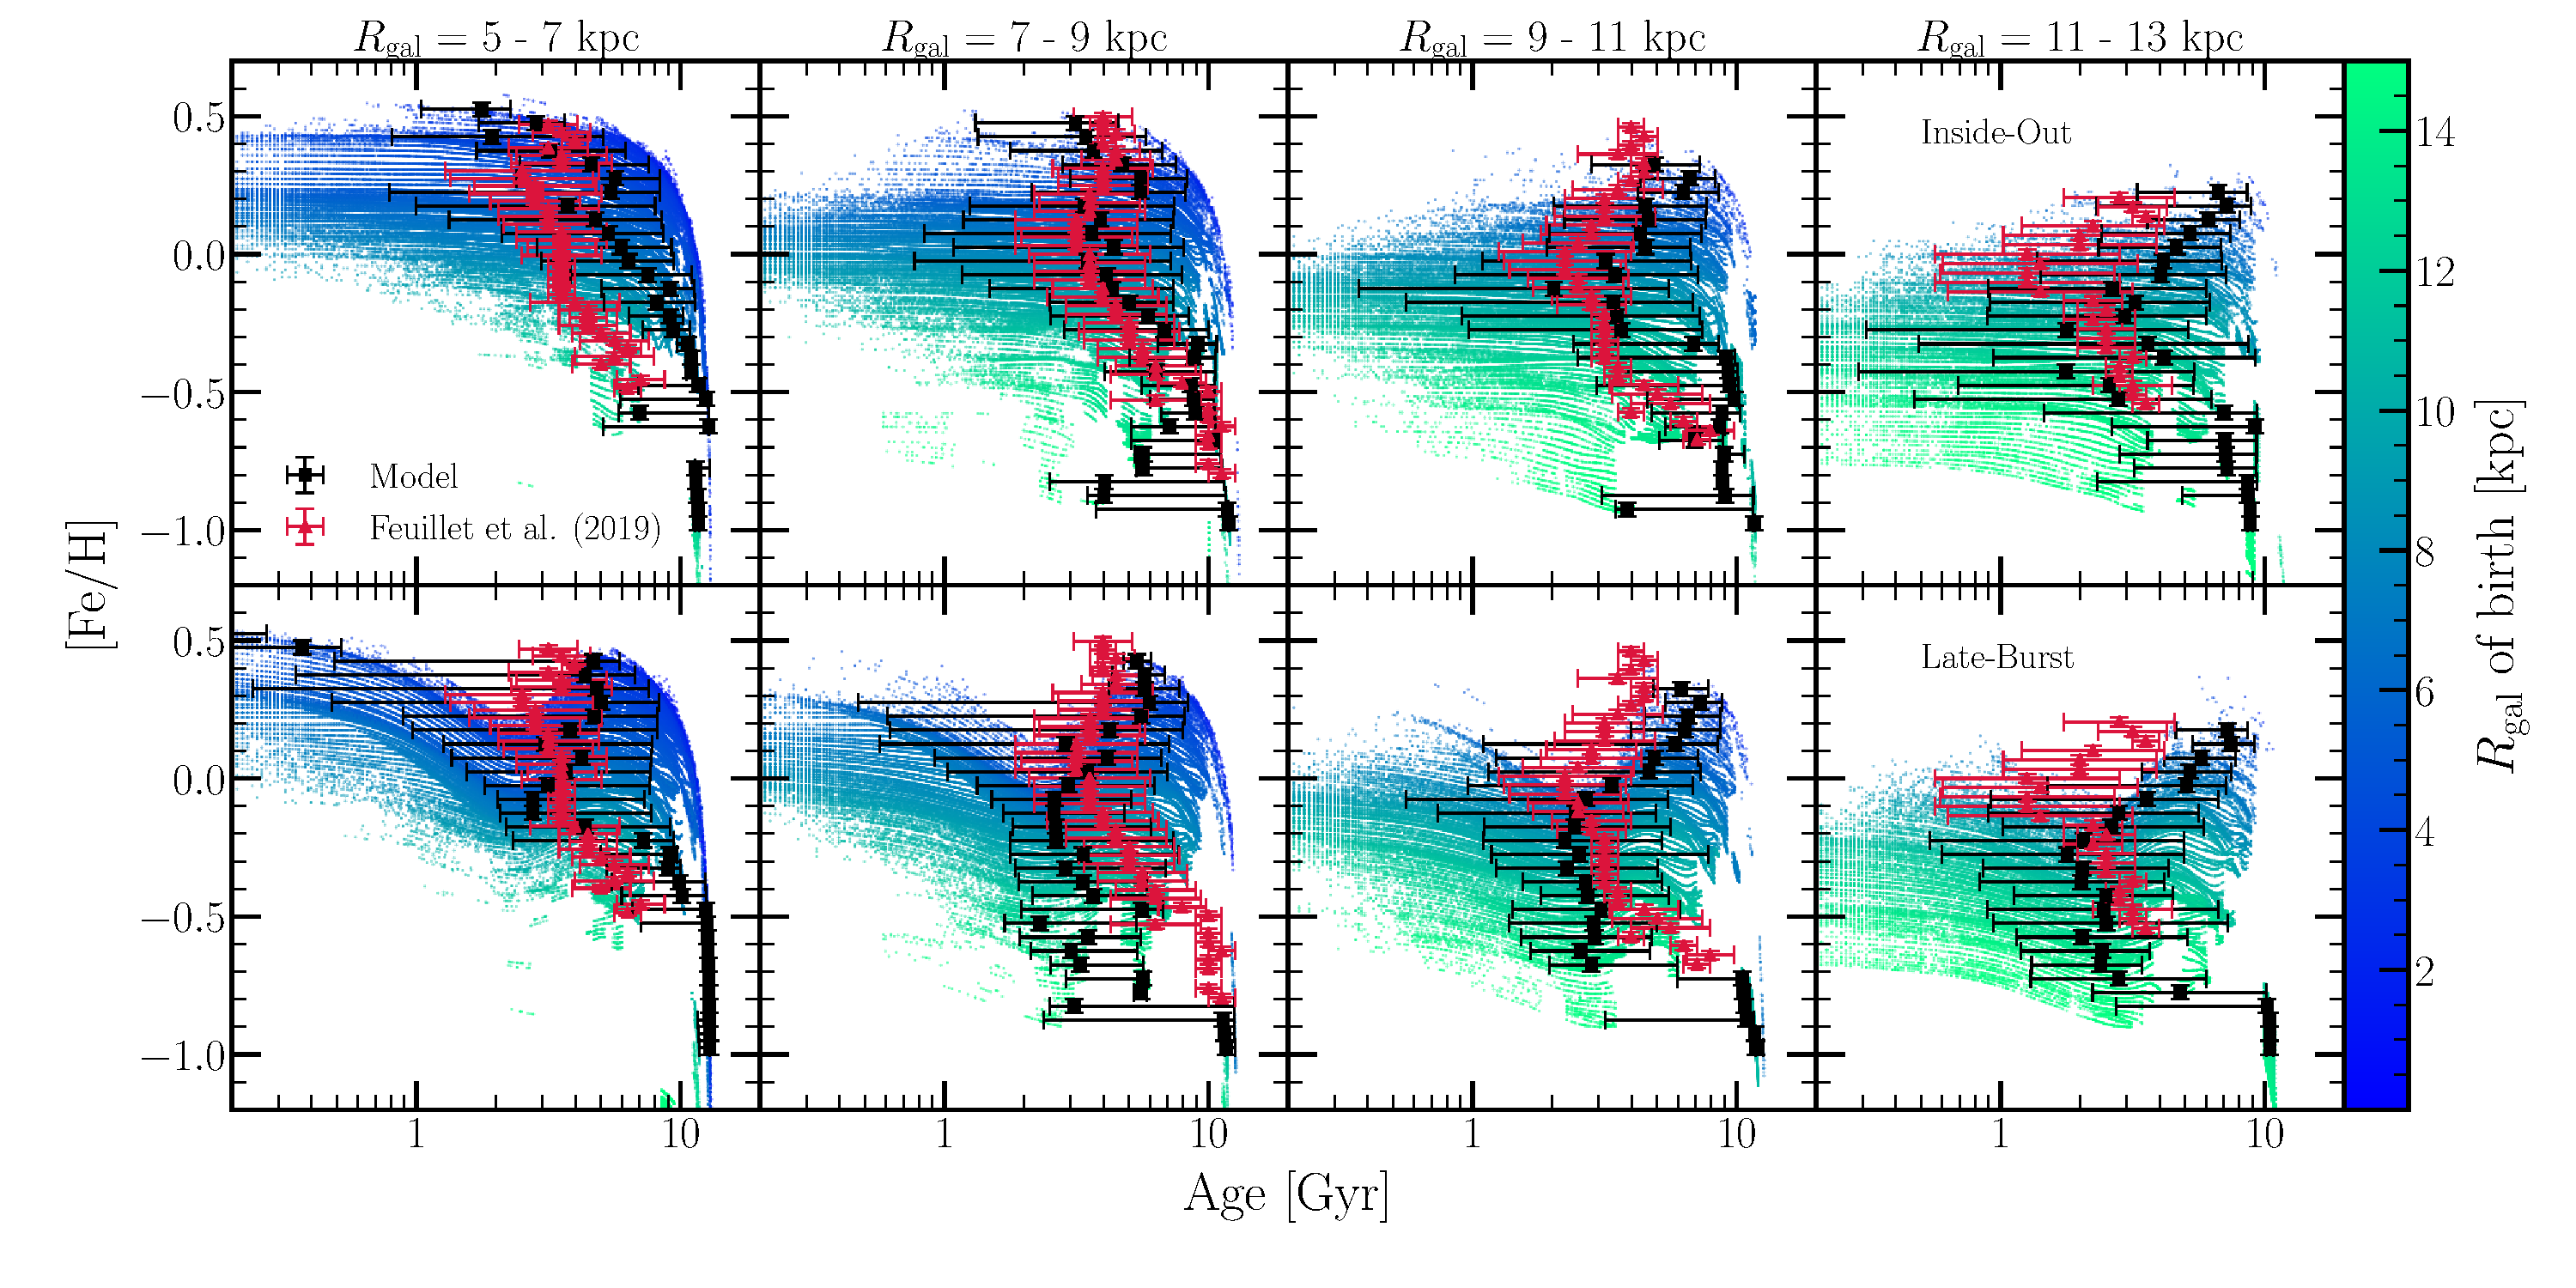
\includegraphics[scale = 0.4]{amr_insideout_vs_lateburst_fe.pdf} 
\caption{The age-[Fe/H] relation predicted by our inside-out (top) and 
late-burst (bottom) SFH models for~$R_\text{gal}$ = 5 - 7 kpc (left), 7 - 9 kpc 
(left middle), 9 - 11 kpc (right middle), and 11 - 13 kpc (right). Each panel 
shows only the~$\left|z\right|\leq$~0.5 kpc population. Red triangles, black 
squares, error bars, and coloured points are as in Fig.~\ref{migration:fig:age_alpha} for 
the corresponding Galactic region, but with the model prediction quantified in 
bins of~$\Delta$[Fe/H] = 0.05. } 
\label{migration:fig:amr_insideout_vs_lateburst_fe} 
\end{figure*} 
\end{landscape}
\clearpage
}

Although the AMR is usually formulated in terms of 
[Fe/H], it is also interesting to quantify the age-[O/H] relation because it 
is not affected by SN Ia enrichment. 
The extent to which the two AMRs differ indicates the extent to which the 
delayed timescale and impact of migration on SN Ia enrichment are important in 
shaping the age-[Fe/H] relation. 
Fig.~\ref{migration:fig:age_oh_static} presents the age-[O/H] relation predicted by our 
constant SFR model for the~$\left|z\right|\leq$~0.5 kpc population at 
$R_\text{gal}$ = 7 - 9 and 11 - 13 kpc. 
The black squares with error bars denote the mass-weighted median age as 
in~\S~\ref{migration:sec:obs_comp:age_alpha}, and we again plot the individual stellar 
populations in the background for reference, colour-coded according to their 
Galactocentric radius of birth. 
We omit the~\citet{Feuillet2019} measurements from this figure but present 
observational comparisons for our more empirically motivated inside-out SFH 
model below. 
The constant SFR model allows us to isolate the effects of stellar migration 
from the time-dependent SFR. 
\par 
The intrinsic scatter in the observed AMR has previously been interpreted as 
evidence for radial mixing~\citep{Edvardsson1993, Sellwood2002}. 
In the solar neighbourhood,~\citet{Feuillet2018} demonstrate that the most 
metal-rich stars tend to be significantly older than solar metallicity stars. 
Using the \citet{Weinberg2017b} analytic models of one-zone chemical evolution 
coupled to a simplified recipe for radial mixing, they argue that this 
non-monotonic trend is the result of old stars born at small~\rgal~where the 
equilibrium abundance is high. 
Only the old stars are able to migrate to the solar neighbourhood due to the 
time required for such a change in their orbital radius. 
\par 
Fig.~\ref{migration:fig:age_oh_static} demonstrates this behaviour for our 
simulation-motivated radial migration prescription. Although it is 
observationally advantageous to measure age in bins of abundance because the 
abundance measurements are much more precise, it is conceptually easier to 
understand the model behaviour in terms of abundance spread at a given age. 
In both regions plotted, the youngest stars form with a composition inherited 
from the local ISM, which in this model is reflective of the late-time 
equilibrium abundance. 
At a given age, only stars born in a well-defined region of the 
Galaxy will have had adequate time to migrate to a given present-day radius. 
Since a range of~\rgal~maps directly to a range of metallicity once 
the ISM is close to the equilibrium abundance, this necessitates a maximum 
width of the [O/H] distribution at fixed age. 
With increasing age, the [O/H] distribution then gets wider because any given 
present-day radius samples stars formed at a wider range of~\rgal. 
We see this effect in Fig.~\ref{migration:fig:age_oh_static}, with the colour-coding of 
the background points making it clear that stellar migration 
is the culprit. 
In the outer Galaxy, virtually all old stars added by migration lie above the 
local equilibrium metallicity. 
In the~\rgal~= 11 - 13 kpc region, our constant SFR model predicts a nearly 
monotonic increase of median population age with increasing [O/H], from 
[O/H] = -0.5 to +0.3. 
This trend is entirely backwards from that expected by simple one-zone models 
of GCE. 
\par 
Fig.~\ref{migration:fig:amr_solar_annulus} compares the age-[O/H] (top) and 
age-[Fe/H] (bottom) relations predicted by our inside-out SFH model for the 
solar neighbourhood (\rgal~= 7 - 9 kpc and \absz~$\leq$ 0.5 kpc) to the 
measurements from \citet{Feuillet2019}. 
For reference, we add the solid dark red line, which denotes the AMR measured 
by~\citet{Feuillet2018}. 
Although our model shows reasonable agreement with the~\citet{Feuillet2019} 
measurements in the solar annulus,~\citet{Feuillet2018} report ages for solar 
metallicity that are considerably younger ($\sim$1 - 2 Gyr as opposed to 
$\sim$3 - 4 Gyr). 
The origin of this difference is not clear, nor is it clear which AMR 
measurement is more reliable (D. Feuillet, private communication). 
Predictions for the inside-out SFH are similar to those shown previously 
for the constant SFR model, demonstrating that radial migration plays a larger 
role than the detailed SFH in determining the qualitative form of the AMR. 
The age-[O/H] and age-[Fe/H] relations are similar for both observations and 
models, a non-trivial result given the different time profile of SN Ia 
enrichment. 
Agreement between the model and the data is somewhat better for [O/H] than for 
[Fe/H]. 
The model predicts a large spread in age at fixed metallicity, comparable to 
but somewhat larger than the spread esimated by~\citet{Feuillet2019}. 
\par
Fig.~\ref{migration:fig:amr_insideout_vs_lateburst_fe} compares the predictions of the 
inside-out (top) and late-burst (bottom) SFH models to the~\citet{Feuillet2019} 
age-[Fe/H] relation in four~\rgal~annuli, always with~\absz~$\leq$ 0.5 kpc. 
% While neither model reproduces the data perfectly, the agreement is better 
% overall for the late-burst model, a difference that is more evident from 
% looking at all four annuli rather than the solar neighbourhood alone. 
% {\color{red} 
At~\rgal~= 5 - 7 kpc, the inside-out model overpredicts the ages of solar and 
sub-solar metallicity stars, an issue which is mitigated by the late-burst 
model. 
The late-burst of star formation reduces the median age of these stars, 
typically by 1 - 2 Gyr, simply because more young stars form with the burst 
than without. 
The late-burst model also more convincingly reproduces the C-shaped AMR, the 
most striking qualitative feature of the observations. 
% } 
The median age of the highest metallicity stars increases because the enhanced 
pristine gas accretion that fuels the starburst (see Fig.~\ref{migration:fig:evol}) 
dilutes the ISM metallicity, an effect that is evident in the tracks for a 
given birth~\rgal~in the lower panels. 
Stars from the inner Galaxy that form during the burst do so at roughly solar 
metallicity rather than appearing in the [Fe/H] = 0.2 - 0.5 bins. 
% {\color{red} 
Both the increase in ages for the most metal-rich stars and decrease in ages 
for solar and sub-solar metallicity stars contribute to the late-burst model 
reproducing this C-shape better than the inside-out model. 
The top two rows of Fig.~\ref{migration:fig:age_oh_comparison} in 
Appendix~\ref{migration:sec:age_oh_relation} present the same comparison for the 
age-[O/H] relation, which is unaffected by SN Ia enrichment. 
The late-burst model improves upon the inside-out model there for the same 
reasons as in age-[Fe/H], but perhaps more clearly when comparing bin-by-bin. 
% Although none of these models reproduce the data perfectly, the detailed form 
% of the AMR in our models is sensitive to the nature of the recent starburst or 
% lackthereof, and its true form was likely more complicated than our 
% parameterization. 
% } 
\par 
% The late-burst of star formation reduces the median age of [Fe/H]~$\approx$ 0 
% stars, typically by 1 - 2 Gyr. 
% The median age of the highest metallicity stars increases because the 
% enhanced pristine gas accretion that fuels the starburst (see Fig. 
% \ref{migration:fig:evol}) dilutes the ISM metallicity, an effect that is evident in the 
% tracks for a given birth~\rgal~in the lower panels. 
% Stars from the inner Galaxy that form during the burst do so at roughly solar 
% metallicity rather than appearing in the [Fe/H] = 0.2 - 0.5 bins. 
% With reduced median age at [Fe/H]~$\approx$ 0 and increased median at 
% [Fe/H] > 0.2, the late-burst model more consistently reproduces the C-shaped 
% AMR that is the most striking qualitative feature of the observations. 
The CCSN and SN Ia associated with the burst also boost the evolutionary 
tracks of the inner Galaxy to higher [Fe/H] at late times, so the predicted 
age distribution at high [Fe/H] is bimodal, especially at~\rgal~= 5 - 7 kpc. 
The~\citet{Feuillet2019} results do not support this dichotomy, but they 
model the observations with the assumption of a Gaussian log age distribution, 
so it is worth returning to the data with the possibility of bimodal age 
distributions in mind. 
% \par 
% {\color{red} 
The outer-burst model, illustrated for the age-[O/H] relation in the bottom 
row of panels in Fig.~\ref{migration:fig:age_oh_comparison} in 
Appendix~\ref{migration:sec:age_oh_relation}, mitigates this issue since it lacks the 
burst at small~\rgal, predicting ages for the most metal-rich stars more in line 
with the~\citet{Feuillet2019} measurements. 
% }
% The outer-burst model mitigates this issue since it lacks the burst at small 
% \rgal, predicting ages for the most metal-rich stars more in line with the 
% \citet{Feuillet2019} measurements. 
% We illustrate this difference in Fig.~\ref{migration:fig:age_oh_comparison} in 
% Appendix~\ref{migration:sec:age_oh_relation} for the age-[O/H] relation. 
% The detailed form of the AMR in our models is sensitive to the nature of the 
% recent starburst, and its true form was likely more complicated than our 
% parameterization. 
% Fig.~\ref{migration:fig:age_oh_comparison} also includes a comparison of the inside-out 
% and late-burst model predictions, now without the effect of SN Ia enrichment. 
% The late-burst model improves upon the inside-out model in age-[O/H] for the 
% same reasons as in age-[Fe/H], but perhaps more clearly when looking 
% bin-by-bin. 
% We do not believe these conclusions are impacted by further discrepancies 
% between any individual model and the observational sample, because our models 
% are not designed to reproduce the data exactly. 
\par 
The late-burst model is motivated by the star formation histories inferred 
empirically by~\citet{Isern2019} and~\citet{Mor2019}. 
Adding this late time enhancement to star formation improves agreement with the 
\citet{Feuillet2019} data, but it is not enough to reproduce the very young 
(< 2 Gyr) median ages of solar metallicity stars found by~\citet{Feuillet2018}. 
If future analyses confirm the 2018 ages rather than the 2019 ages, they would 
require a later and more extreme starburst to explain them. 
As discussed in~\S~\ref{migration:sec:obs_comp:age_alpha}, the late-burst 
\textit{worsens} agreement with the~\citet{Feuillet2018, Feuillet2019} 
age-[O/Fe] relation because of the increased [O/Fe] at late times (see Fig. 
\ref{migration:fig:age_alpha}). 
We do not see an obvious way to achieve good simultaneous agreement with the 
observationally inferred SFH, the age-[O/Fe] relation, and the age-[Fe/H] 
relation. 
Possibly a well-tuned choice of yields and the temporal and radial range of 
the burst could achieve such agreement; it is possible that the latter is 
related to the spatial dependence of the age-[O/Fe] relation seen in 
the~\citet{Feuillet2019} data (see Fig.~\ref{migration:fig:age_alpha_regions}). 
Alternatively, an outflow prescription that preferentially removes CCSN 
ejecta rather than ambient ISM~\citep[see, e.g.,][]{Vincenzo2016b,
Chisholm2018, Christensen2018} could mitigate the increase in [O/Fe] during
the burst (such a 
prescription is physically plausible, but it would require a wholesale 
recalibration of our model parameters). 
For now we conclude that radial migration can naturally explain otherwise 
puzzling features of the AMR and that evidence for enhanced late-time star 
formation in the Milky Way is ambiguous. 
Age-abundance relations are clearly a powerful diagnostic of GCE models, and 
observational investigations that demonstrate consistency across age 
determination methods, probe the shape of the age distribution at fixed 
abundance, and extend still further across the disc are highly desirable. 

